%!TEX root = ../thesis.tex
\chapter[Diffusion MRI protocols for single fibre structures]{Optimized diffusion MRI protocols for estimating axon diameter with known fibre orientation}
% Define box and box title style
\tikzstyle{protocolbox} = [draw=black, thin, rectangle, rounded corners, inner xsep=5pt, outer ysep=0pt] \tikzstyle{protocolheader} = [draw=none, fill=gray!30, rounded corners, inner sep = 5pt] \tikzstyle{protocoltext} = [draw=black, fill=white, rounded corners, inner sep = 5pt]

\newcommand{\SF}{{\ensuremath{\mathcal{SF}}}}
\newcommand{\OI}{{\ensuremath{\mathcal{OI}}}}
\newcommand{\SD}{{\ensuremath{\mathcal{SF}_{pulses}}}}
\newcommand{\DO}{{\ensuremath{\mathcal{SF}_{dirs}}}}
\newcommand{\FD}{{\SF}}







% Diffusion analysis techniques can be seen as trade-off between model complexity and amount of data needed. In this context, the two techniques we have investigated in the previous chapters DTI and QSI might be regarded as two opposite ends of this trade-off. DTI only requires relatively little amounts of data ( minimum 6 different gradient directions + 1 non-diffusion weighted acquisition), but it's underlying model is based on the assumption that all observed diffusion is Gaussian. Clearly, this is a gross over-simplification of the complex diffusion mechanisms present in biological tissue. QSI on the other end of this spectrum makes no assumption about the diffusion process and can theoretically reveal even the most complex diffusion displacement profiles. As a trade-off for this generality, QSI generally required large quantities of data and requires very strong diffusion gradients. In fact the implementation of true QSI on a clinical systems is impossible, and quasi-QSI type acquisitions are subject to their own approximations and shortcomings (see Chapter XX for discussion). Model-based diffusion imaging techniques are a compromise between the model-free techniques and simple models such as DTI (see Chapter XX). The data requirements for these model range from single shell HARDI (e.g. Ball-and-Stick models) comparable to DTI up to multiple shell HARDI or QSI type protocols. Furthermore, geometrical models offer the potential to discriminate different tissue compartments better than DTI, while its parameters can be more easy to interpret than the PDF derived from QSI.
%
% The protocol optimisation approach of \citep{TODO} provides a computational framework that can automatically determine the optimal set of parameters for a specific model-based imaging approach, also taking into account the technical cornerstones of the MRI setup, i.e., maximum available gradient strength, SNR of the images and available scan time. The optimisation in \citep{TODO} was designed independent of the underlying fibre orientation as it was aimed towards whole brain imaging.

In the previous chapters we have investigated two very different techniques in \gls{DTI} and \gls{QSI}. \gls{DTI} only requires relatively little amounts of data, but it's underlying model is based on the assumption that all observed diffusion is Gaussian. Clearly, this is a gross over-simplification of the complex diffusion mechanisms present in biological tissue. \gls{QSI} on the other hand makes no assumption about the diffusion process and can theoretically reveal even the most complex diffusion displacement profiles. \gls{QSI} generally requires large amounts of data and requires very strong diffusion gradients. Henceforth, the implementation of true \gls{QSI} on clinical systems is very difficult and the derived parameters are often difficult to interpret (see Chapter \ref{next chap}).
\paragraph{}
In the following chapters we will investigate a different model-based diffusion imaging technique, which can be seen as a compromise between the simple model of \gls{DTI} and the complex \gls{QSI} approach. Here, our work is heavily based on the ActiveAx approach by \citet{Alexander:2008}, who used a simple compartment tissue model to derive axon diameter and axon density indices in the brain using standard clinical hardware (see Chapter\ref{ref}).


Alexander's work is designed under the premise of full brain imaging and therefore he presents DWI protocols that work independently of the fibre orientation. We call this the orientation invariant ({\OI}) approach. The {\OI} approach is based on acquiring multiple HARDI shells and requires good angular resolution to retain the orientation invariant features. As a consequence, the {\OI} protocols used e.g. in \citep{Alexander:2010} require scan times of more than 1h, which limits their transition to clinical practise.


The main motivation of this work is to reduce the scan time of the ActiveAx protocols to a more clinically applicable limit of 20-30 minutes. The central idea to attain this reduction is to discard the requirement for orientational invariance and focus on structures with a coherent known single fibre orientation. Many studies before have focussed on those single fibre structures (e.g. \gls{CC} or \gls{SC}) as they can be expressed in terms of relatively simple models, without the need to include complex fibre configurations such as multiple fibre crossings, bending or fanning. Furthermore, many single fibre structures such as \gls{CC} and \gls{SC} are of great importance to many developmental and pathological processes. Our approach makes imaging these structures more practicable with a 20-30 minute time frame, where a >1h full-brain protocol might not be feasible.
\paragraph{}
In this chapter, we present a modification to the existing protocol optimization framework of \cite{Alexander:2008} (see Section~\ref{sec:protocol_optimisation}) that incorporates this \textit{a-priori} information about fibre organisation. We refer to this approach and its resulting protocols as the single-fibre ({\SF}) method. We evaluate different {\SF} implementations and use computer simulations to test and compare the \SF method to the {\OI} approach. By design, the {\SF} is optimised only for a specific predetermined fibre orientation. However, in reality there will always be some variation even in very coherently aligned \gls{WM} tracts. We therefore test how much influence this variation has on our {\SF} approach compared to {\OI}. Finally, we implemented the {\SF} protocol to demonstrate its feasibility within a real biological tissue sample of fixed cervical monkey \gls{SC}. Although this study is motivated by improving in-vivo clinical applicability, we chose to first test our approach on a pre-clinical scanner on a fixed tissue sample to avoid the challenges of in-vivo scanning (e.g. motion and insufficient image resolution) and focus on an initial demonstration of our method. The results and observations made in this chapter form the basis of the subsequent in-vivo implementation we present in the following chapter.

\section{Protocol optimisation}
This section discusses how we adapt the {\OI} optimisation of \citet{Alexander:2008} to the {\SF} case. The original {\OI} optimisation is designed to determine the best PGSE pulse parameters (i.e. \gls{gstr}, \gls{smalldel}, \gls{bigdel}) for a fixed number $M$ of shells, each including a fixed number $N$ of distributed gradient directions. The gradient directions scheme in the \OI{} approach is fixed and uniformly distributed over the sphere as in \citep{Cook:2007}. The HARDI-like gradient scheme is necessary to guarantee orientational invariance, i.e. be sensitive to restriction regardless of diffusion direction. In our {\SF} implementation we can assume a known diffusion direction and therefore do not require the uniform angular sampling of the {\OI} approach. This allows us to include the gradient scheme to together with the PGSE pulse setting in the optimisation process. In addition to {\SF}, which optimises gradient scheme and PGSE pulse parameters simultaneously, we are also interested in how much the optimisation of the gradient scheme ({\DO}) alone and the PGSE parameters alone ({\SD}) has on the performance of the resulting protocols. In total we tested the four following different variants of \citet{Alexander:2008}'s optimisation framework:

\begin{description}
	\item[\OI:] The orientationally invariant protocol optimisation as described in \citep{Alexander:2008}.
	\item[\FD:] The adapted algorithm optimises both the PGSE parameters and gradient direction scheme for $M$ shells assuming a single \textit{a-priori} known fibre direction.
	\item[\SD:] Similar to the {\OI} optimisation approach, the algorithm uses a fixed gradient scheme for each of the $M$ shells and only optimises the PGSE pulse parameters. The main difference to \OI{} is that the algorithm optimises for a single \textit{a-priori} known fibre direction instead of a set of \lq worst case\rq fibre directions.
	\item[\DO:] This is a two-step optimisation approach. The {\SD} algorithm is performed to determine the best $M$ PGSE pulse settings. In a second step the gradient scheme for each of the each $M$ shells are optimised, keeping the PGSE pulse parameters fixed.
\end{description}

Table~\ref{tab:chapter7 exp1 opt parameter overview} summarises the optimisation parameters for each of the four algorithms. It is important to note that the inclusion of the optimisation of individual gradient directions in {\DO} and {\FD} drastically increases the number of free parameters to be optimised from $O(M)$ to $O(N\cdot M)$ compared to {\OI} and {\SD}.
\begin{table}[th]
  	\caption{Overview of parameters for the tested protocol optimisation approaches.} \centering \vspace{2ex}
    \label{tab:chapter7 exp1 opt parameter overview}
    \begin{adjustbox}{width={\textwidth},totalheight=\textheight,keepaspectratio}
        	\begin{tabular}
        		{@{}y{0.35\textwidth}x{0.2\textwidth}x{0.2\textwidth}x{0.2\textwidth}x{0.2\textwidth}x{0.15\textwidth}@{}}
                \toprule
                Protocol name & {\OI} & {\FD} & {\SD} & {\DO}  \\%
        		& \footnotesize{(orientation invariant)} & \footnotesize{(pulses + directions)} & \footnotesize{(pulses only)} & \footnotesize{(directions only)} \\%
        		\cmidrule(r){2-2} \cmidrule(rl){3-3} \cmidrule(rl){4-4} \cmidrule(l){5-5} Free parameters & $\delta_m,\Delta_m,G_m$ & $\phi_{m,n},\theta_{m,n}$ &  $\delta_m,\Delta_m,G_m$ & $\phi_{m,n},\theta_{m,n}$ \\
        		& & $\delta_m,\Delta_m,G_m$ & &  \\[1.5ex]
        		Fixed parameters & $\phi_n,\theta_n$ & -- & $\phi_n,\theta_n$ & $\delta_m,\Delta_m,G_m$  \\[2ex]
        		Specific fibre direction & no & yes & yes & yes \\[2ex]
        		No. of free parameters & O($M$) & O($M\times N)$ &O($M$) & O($M\times N$) \\
        		\bottomrule
        	\end{tabular}        	
    \end{adjustbox}
\end{table}

\subsection{Tissue model}
   Like \citep{Alexander:2008}, we use a simple two-compartment model of white matter tissue, with axons represented as cylinders with a single radius and extra-axonal tissue represented by an axially symmetric diffusion tensor ('ZeppelinCylinder' in the taxonomy of \cite{Panagiotaki:2012}).  For the optimisation we assume tissue diffusion properties typically found in \emph{in-vivo} human white matter. A full list of the model parameters used in the optimisation is given in Table~\ref{tab: chapter7 exp1 model opt parameters clinical}.

\begin{table}[!ht]
	\caption{Model parameters used for optimisation.}
    \centering
    \vspace{2ex}	
    % Cylinder
    \begin{tabular}{y{0.1\textwidth}y{0.25\textwidth}}
    \addlinespace
    \toprule
    \multicolumn{2}{c}{\textbf{Cylinder}} \\
    \multicolumn{2}{c}{(intra-axonal)} \\
    \midrule
    $f_{intra}$ & $0.7$ \\
    $D_{\|}$ & $1.7\cdot 10^{-9}$ $s/mm^2$ \\
    $D_{\bot} $ & $6\cdot 10^{-10}$ $s/mm^2$ \\
    dir   & $[0,0,1]^T$ \\
    R & $\{1..1..10\}\mu m$ \\
    \bottomrule
    \end{tabular}%
    \hspace{0.15\textwidth}
    %%% Zeppelin
    \begin{tabular}{y{0.1\textwidth}y{0.25\textwidth}}
    \addlinespace
    \toprule
    \multicolumn{2}{c}{\textbf{Axially symmetric tensor}} \\
    \multicolumn{2}{c}{(extra-axonal)} \\
    \midrule
    $f_{extra}$& $0.3$ \\
    $D_{\parallel}$ & $1.7\cdot 10^{-9}$ $m^2/s$ \\
    $D_{\bot} $ & $6\cdot 10^{-10}$ $s/m^2/s$ \\
    dir & $[0,0,1]^T$ \\
    \bottomrule
    & \\ %empty line to level tables
    \end{tabular}%
    \label{tab: chapter7 exp1 model opt parameters clinical}
    \vspace{2ex}	
\end{table}

\subsection{Implementation}
We implement the four algorithms as described in Section~\ref{XX}  for $M=8$ different sets of PGSE parameters. For for {\OI} and {\SD} we use the default setting for the SOMA algorithm , i.e., 500 migration steps with 100 migrating individuals. For {\DO} and {\SD}, the parameter space to explore is much larger and we are using 1000 individuals with 750 migration steps to ensure convergence. To avoid local minima, each optimisation is repeated 5 times and from the resulting protocols the one with the smallest CRLB is chosen. The available gradient strength is limited to 60mT/m to simulate a typical clinical MRI scanner.

\subsection{Optimised protocols}
\paragraph{}
Figure~\ref{fig:chapter7 exp1 DIRS vs CRLB} shows the CRLB of the four different optimisation for different $N$. We can see that CRLB distinguishes the four protocols in two groups: {\OI}/{\SD} with fixed directions and {\DO}/{\FD} with optimised directions. {\DO} and {\FD} consistently produce lower CRLB than {\OI} and {\SD} regardless of the chosen $N$, although the differences between the two groups become smaller for larger $N > 60$. For better comparison, Figure~\ref{fig:chapter7 exp1 DIRS vs CRLB} shows the corresponding $N$ for a different values of CRLB. We can see that {\FD} and {\DO} both achieve the same CRLB values of {\OI} with significantly less directions. In other words, the {\DO} and {\FD} promise a comparable performance to {\OI} with only 25\%--33\% the amount of data required.

\begin{figure}[H]
	\centering
	\begin{tikzpicture}
	\begin{axis}[
	  		xlabel={SNR},
			ylabel={CRLB},
            xmajorgrids=true,
            ymajorgrids=true,
            width=0.9\textwidth,
            height=0.5\textwidth,
	  		%xmin=-3.2,
	  		%xmax=3.2,
	  		xtick={10,20,30,40,50},
	  		%xticklabels={$-\pi$,$-\frac{\pi}{2}$,0,$\frac{\pi}{2}$,$\pi$},
	  		%ymin=0,
	  		%ymax=1.5708,
	  		%ytick={0,0.7854,1.5708},
	  		%yticklabels={0,$\frac{\pi}{4}$,$\frac{\pi}{2}$}
			ybar,				
	  	]
	  	\addplot+[red, mark options={fill=red}] table[x=SNR,y=nofib] {chapter7/figs/SNRvsCRLB_60mT.txt};
		\addplot+[green, mark options={fill=green}] table[x=SNR,y=samedir] {chapter7/figs/SNRvsCRLB_60mT.txt};
		\addplot+[blue, mark options={fill=blue}] table[x=SNR,y=dironly] {chapter7/figs/SNRvsCRLB_60mT.txt};
		\addplot+[cyan, mark options={fill=cyan}] table[x=SNR,y=free] {chapter7/figs/SNRvsCRLB_60mT.txt};
		\legend{\OI, \SD, \DO, \FD};
	\end{axis}
\end{tikzpicture}	

	%\begin{tikzpicture}	
	\begin{axis}[
            title={\textbf{Pre-clinical protocol} $(|G_{max}|=300mT/m)$},
	  		xlabel={SNR},
			ylabel={CRLB},
            xmajorgrids=true,
            ymajorgrids=true,
            width=0.45\textwidth,
            %height=0.4\textwidth,
	  		%xmin=-3.2,
	  		%xmax=3.2,
	  		%xtick={-3.1416,-1.5708,0,1.5708,3.1416},
	  		%xticklabels={$-\pi$,$-\frac{\pi}{2}$,0,$\frac{\pi}{2}$,$\pi$},
	  		%ymin=0,
	  		%ymax=1.5708,
	  		%ytick={0,0.7854,1.5708},
	  		%yticklabels={0,$\frac{\pi}{4}$,$\frac{\pi}{2}$}				
	  	]
	  	\addplot+[red, mark options={fill=red}] table[x=SNR,y=nofib] {chapter7/figs/SNRvsCRLB_300mTCopenhagen.txt};
		\addplot+[green, mark options={fill=green}] table[x=SNR,y=samedir] {chapter7/figs/SNRvsCRLB_300mTCopenhagen.txt};
		\addplot+[blue, mark options={fill=blue}] table[x=SNR,y=dironly] {chapter7/figs/SNRvsCRLB_300mTCopenhagen.txt};
		\addplot+[cyan, mark options={fill=cyan}] table[x=SNR,y=free] {chapter7/figs/SNRvsCRLB_300mTCopenhagen.txt};
		\legend{\OI, \SD, \DO, \FD};
	\end{axis}
\end{tikzpicture}	
	\caption{CRLBs of optimised protocols under different SNR.}
	\label{fig:chapter7 exp1 SNR vs CRLB}
\end{figure}

Figure~\ref{fig:chapter7 exp1 SNR vs CRLB} shows the CRLB of the four different optimisations for a fixed $N=90$ but different SNR conditions. The results here are very similar to the findings shown above. Both {\FD} and {\DO} consistently show CRLB values three to four times lower than those of {\OI} and {\SD} for similar SNR values. The differences are most apparent for low SNR values, which are also more common in real clinical diffusion MRI.
\begin{figure}[H]
	\centering
	\begin{tikzpicture}	
	\begin{axis}[
            title={\textbf{Clinical protocol} $(|G_{max}|=60mT/m)$},
            ymajorgrids=true,
	  		xlabel={\#Gradient directions per set},
			ylabel={CRLB},
            width=0.9\textwidth,
            height=0.5\textwidth,
	  		xtick={15,30,35,45,60,75,90,105,120},
	  		xticklabels={15,\color{red}{30},\color{red}{35},\color{red}{45},60,75,90,105,120},
            xmin=0,
            xmax=120,
            ymin=0,
	  		%ytick={0,0.7854,1.5708},
	  		%yticklabels={0,$\frac{\pi}{4}$,$\frac{\pi}{2}$},				
	  	]
	  	\addplot+[very thick, red, mark options={fill=red}] table[x=DIRS,y=nofib] {chapter7/figs/DIRSvsCRLB_60mT.txt};
		\addplot+[very thick, green, mark options={fill=green}] table[x=DIRS,y=samedir] {chapter7/figs/DIRSvsCRLB_60mT.txt};
		\addplot+[very thick, blue, mark options={fill=blue}] table[x=DIRS,y=dironly] {chapter7/figs/DIRSvsCRLB_60mT.txt};
		\addplot+[very thick, cyan, mark options={fill=cyan}] table[x=DIRS,y=free] {chapter7/figs/DIRSvsCRLB_60mT.txt};
        %75 OI vs FD
        \addplot[thick,dashed, black,sharp plot,update limits=false] coordinates {(30,0.38) (75,0.38)};
        \addplot[thick,dashed, black,sharp plot,update limits=false] coordinates {(30,0) (30,0.38)};
        %90 OI vs FD
        \addplot[thick,dashed, black,sharp plot,update limits=false] coordinates {(35,0.32) (90,0.32)};
        \addplot[thick,dashed, black,sharp plot,update limits=false] coordinates {(35,0) (35,0.32)};
        %120 OI vs FD
        \addplot[thick,dashed, black,sharp plot,update limits=false] coordinates {(45,0.2379) (120,0.2379)};
        \addplot[thick,dashed, black,sharp plot,update limits=false] coordinates {(45,0) (45,0.2379)};
		\legend{\OI, \SD, \DO, \FD};
	\end{axis}
\end{tikzpicture}	

	%\begin{tikzpicture}	
	\begin{axis}[
            title={\textbf{Pre-clinical protocol} $(|G_{max}|=300mT/m)$},
            ymajorgrids=true,
	  		xlabel={\#Gradient directions per set},
			ylabel={CRLB},
            width=0.9\textwidth,
            height=0.6\textwidth,
	  		xtick={15,30,35,45,60,75,90,105,120},
	  		xticklabels={15,\color{red}{30},\color{red}{35},\color{red}{45},60,75,90,105,120},
            xmin=0,
            xmax=120,
            ymin=0,
	  		%ytick={0,0.7854,1.5708},
	  		%yticklabels={0,$\frac{\pi}{4}$,$\frac{\pi}{2}$}				
	  	]
	  	\addplot+[very thick, red, mark options={fill=red}] table[x=DIRS,y=nofib] {chapter7/figs/DIRSvsCRLB_300mTCopenhagen.txt};
		\addplot+[very thick, green, mark options={fill=green}] table[x=DIRS,y=samedir] {chapter7/figs/DIRSvsCRLB_300mTCopenhagen.txt};
		\addplot+[very thick, blue, mark options={fill=blue}] table[x=DIRS,y=dironly] {chapter7/figs/DIRSvsCRLB_300mTCopenhagen.txt};
		\addplot+[very thick, cyan, mark options={fill=cyan}] table[x=DIRS,y=free] {chapter7/figs/DIRSvsCRLB_300mTCopenhagen.txt};
        %75 OI vs FD
        \addplot[thick,dashed, black,sharp plot,update limits=false] coordinates {(30,0.31) (75,0.31)};
        \addplot[thick,dashed, black,sharp plot,update limits=false] coordinates {(30,0) (30,0.31)};
        %90 OI vs FD
        \addplot[thick,dashed, black,sharp plot,update limits=false] coordinates {(35,0.26) (90,0.26)};
        \addplot[thick,dashed, black,sharp plot,update limits=false] coordinates {(35,0) (35,0.26)};
        %120 OI vs FD
        \addplot[thick,dashed, black,sharp plot,update limits=false] coordinates {(45,0.2) (120,0.2)};
        \addplot[thick,dashed, black,sharp plot,update limits=false] coordinates {(45,0) (45,0.2)};
		\legend{\OI, \SD, \DO, \FD};
	\end{axis}
\end{tikzpicture}	

	\caption{CRLBs of optimised protocols with different $N$  number of gradient directions.}
	\label{fig:chapter7 exp1 DIRS vs CRLB}
\end{figure}
\paragraph{}
Table~\ref{fig:chapter7 exp1 protocol 60mT} shows an example of the \OI{} and \SF{} protocols variants we obtain for $N=90$ and SNR$=20$. A more comprehensive visualisation of the different protocol parameters can be found in Appendix~\ref{app:chapter7 protocols 60mT}. We deliberately chose a large number of $M$ to reevaluate the optimal number of different PGSE for each protocol. Our findings here confirm the results of \citep{Alexander:2008}, which suggest that a smaller number of $M=4$ suffices to capture all unique combinations of PGSE pulse parameters. We also note that {\OI} and {\SD} protocols are almost identical, which suggest that the choice of diffusion orientation for the {\OI} has little influence on the outcome of the algorithm.
\begin{table}[H]
\caption{Protocol parameters and gradient schemes for $N=90$, $M=8$. The $M$ different gradient direction schemes are coded by different colors. Please note that in the \OI{} and \SD{} protocols all $M$ gradient direction schemes are identical.}
\label{fig:chapter7 exp1 protocol 60mT}
\begin{adjustbox}{minipage=\linewidth}
\subfloat[\OI protocol]
{
    \begin{minipage}{\textwidth}
    \begin{tabular}{rrrr}
        \addlinespace
        \toprule
        $\delta$ & $\Delta$ & $|G|$ & $b$-value \\
        $[ms]$ & $[ms]$ & $[mT/m]$ & $[s/mm^2]$\\
        \midrule
        12.9  & 17.9  & 60    & 583 \\
        12.9  & 17.9  & 60    & 585 \\
        12.9  & 17.9  & 60    & 587 \\
        12.9  & 17.9  & 60    & 588 \\
        22.7  & 48.3  & 30    & 1480 \\
        24.4  & 46.6  & 30    & 1684 \\
        26.3  & 44.7  & 40    & 2752 \\
        33    & 38    & 60    & 7585 \\
        \bottomrule
    \end{tabular}%
    \hspace{1cm}
        \raisebox{-2cm}{
        \begin{tikzpicture}[scale=0.7]
              \begin{axis}[xmax=1, xmin=-1, ymax=1, ymin=-1, zmax=1, zmin=-1, width=4.0cm, height=4.0cm, grid=major,legend entries={all},cycle multi list={color list\nextlist[2 of]mark list},legend pos=outer north east]
              \addplot3+[only marks] table {chapter7/figs/protocols_par1/SF_OI_60mT001.txt};
        \end{axis}
        \end{tikzpicture}
        }
  \end{minipage}
}


\subfloat[\FD protocol]
{
    \begin{minipage}{\textwidth}
    \begin{tabular}{rrrr}
    \addlinespace
    \toprule
        $\delta$ & $\Delta$ & $|G|$ & $b$-value \\
        $[ms]$ & $[ms]$ & $[mT/m]$ & $[s/mm^2]$\\
        \midrule
        14.7  & 19.8  & 60    & 832 \\
        14.8  & 19.8  & 60    & 837 \\
        15.1  & 20.1  & 60    & 883 \\
        15.4  & 20.4  & 60    & 932 \\
        21.2  & 53.9  & 30    & 1361 \\
        27.2  & 47.9  & 40    & 3123 \\
        27.9  & 47.2  & 40    & 3452 \\
        35    & 40    & 60    & 8974 \\
        \bottomrule
    \end{tabular}%
    \hspace{1cm}
        \raisebox{-2cm}{
        \begin{tikzpicture}[scale=0.7]
              \begin{axis}[xmax=1, xmin=-1, ymax=1, ymin=-1, zmax=1, zmin=0, width=4.0cm, height=4.0cm, grid=major,legend entries={1,2,3,4,5,6,7,8},cycle multi list={color list\nextlist[2 of]mark list},legend pos=outer north east]
              \addplot3+[only marks] table {chapter7/figs/protocols_par1/SF_FD_60mT005.txt};
              \addplot3+[only marks] table {chapter7/figs/protocols_par1/SF_FD_60mT004.txt};
              \addplot3+[only marks] table {chapter7/figs/protocols_par1/SF_FD_60mT003.txt};
              \addplot3+[only marks] table {chapter7/figs/protocols_par1/SF_FD_60mT001.txt};
              \addplot3+[only marks] table {chapter7/figs/protocols_par1/SF_FD_60mT007.txt};
              \addplot3+[only marks] table {chapter7/figs/protocols_par1/SF_FD_60mT008.txt};
              \addplot3+[only marks] table {chapter7/figs/protocols_par1/SF_FD_60mT006.txt};
              \addplot3+[only marks] table {chapter7/figs/protocols_par1/SF_FD_60mT002.txt};
        \end{axis}
        \end{tikzpicture}
        }
    \end{minipage}
}


\subfloat[\SD protocol]
{
  \begin{minipage}{\textwidth}
    \begin{tabular}{rrrr}
        \addlinespace
        \toprule
        $\delta$ & $\Delta$ & $|G|$ & $b$-value \\
        $[ms]$ & $[ms]$ & $[mT/m]$ & $[s/mm^2]$\\
        \midrule
        12.8  & 17.8  & 60    & 572 \\
        12.9  & 17.9  & 60    & 580 \\
        12.9  & 17.9  & 60    & 580 \\
        12.9  & 17.9  & 60    & 582 \\
        21.9  & 48.9  & 30    & 1484 \\
        24.7  & 46    & 30    & 1677 \\
        26.3  & 44.5  & 40    & 2639 \\
        32.9  & 37.9  & 60    & 7515 \\
        \bottomrule
    \end{tabular}%
    \hspace{1cm}
        \raisebox{-2cm}{
        \begin{tikzpicture}[scale=0.7]
              \begin{axis}[xmax=1, xmin=-1, ymax=1, ymin=-1, zmax=1, zmin=-1, width=4.0cm, height=4.0cm, grid=major,legend entries={all},cycle multi list={color list\nextlist[2 of]mark list},legend pos=outer north east]
              \addplot3+[only marks] table {chapter7/figs/protocols_par1/SF_OI_60mT001.txt};
        \end{axis}
        \end{tikzpicture}
        }
  \end{minipage}
}


\subfloat[\DO protocol]
{
    \begin{minipage}{\textwidth}
        \begin{tabular}{rrrr}
            \addlinespace
            \toprule
            $\delta$ & $\Delta$ & $|G|$ & $b$-value \\
            $[ms]$ & $[ms]$ & $[mT/m]$ & $[s/mm^2]$\\
            \midrule
            12.8  & 17.8  & 60    & 572 \\
            12.9  & 17.9  & 60    & 580 \\
            12.9  & 17.9  & 60    & 580 \\
            12.9  & 17.9  & 60    & 582 \\
            21.9  & 48.9  & 30    & 1484 \\
            24.7  & 46    & 30    & 1677 \\
            26.3  & 44.5  & 40    & 2639 \\
            32.9  & 37.9  & 60    & 7515 \\
            \bottomrule
        \end{tabular}%
        \hspace{1cm}
        \raisebox{-2cm}{
        \begin{tikzpicture}[scale=0.7]
              \begin{axis}[xmax=1, xmin=-1, ymax=1, ymin=-1, zmax=1, zmin=0, width=4.0cm, height=4.0cm, grid=major,legend entries={1,2,3,4,5,6,7,8},cycle multi list={color list\nextlist[2 of]mark list},legend pos=outer north east]
              \addplot3+[only marks] table {chapter7/figs/protocols_par1/SF_DO_60mT004.txt};
              \addplot3+[only marks] table {chapter7/figs/protocols_par1/SF_DO_60mT007.txt};
              \addplot3+[only marks] table {chapter7/figs/protocols_par1/SF_DO_60mT003.txt};
              \addplot3+[only marks] table {chapter7/figs/protocols_par1/SF_DO_60mT008.txt};
              \addplot3+[only marks] table {chapter7/figs/protocols_par1/SF_DO_60mT006.txt};
              \addplot3+[only marks] table {chapter7/figs/protocols_par1/SF_DO_60mT001.txt};
              \addplot3+[only marks] table {chapter7/figs/protocols_par1/SF_DO_60mT002.txt};
              \addplot3+[only marks] table {chapter7/figs/protocols_par1/SF_DO_60mT005.txt};
        \end{axis}
        \end{tikzpicture}
        }
    \end{minipage}
}
\end{adjustbox}
\end{table}

\section{Experiments}
\subsection{Synthetic data}
From all protocols for $N=90$ and $SNR=20$ we generate synthetic datasets, with which we then test and compare the performance of the different protocol optimisations. The number of gradient directions was chosen rather large to allow sufficient angular resolution for {\OI} and {\DO} protocols.
\paragraph{}
\label{sec: chapter 6 fibre distribution perfect}.
 The MR signals are generated from the same tissue model and tissue diffusion properties we used for the protocol optimisation (see section \ref{XX} and Table~\ref{XX} for details). We use the Camino software package \citep{Cook:2006} to simulate datasets for four different cylinder radii $R={1,2,5,10}\mu m$ as a representation of radii usually found in \emph{in-vivo} white matter tissue. To simulate noise in the MR acquisition, we add Rician noise with $SNR=20$ to the simulated noise-free datasets. To concentrate on comparing the estimates of radius and volume fraction between the protocols we assume all cylinders to be perfectly aligned along the $[0,0,1]^T$ as assumed in the optimisation process.

\subsubsection*{Effect of principle diffusion direction}
Even in very coherent structures such as the \gls{CC}, the observed fibre direction is subject to some variation. However the protocols {\FD} and {\DO} contain gradient schemes designed for a fixed principle diffusion direction. To test the effect of potential misalignment between assumed and true principal diffusion direction we design the following experiment:
\paragraph{}
We create similar dataset as above, with the exception of varying the principal diffusion direction for each synthetic sample. Using the spherical representation of the cylinder direction, we sample each combination of polar angle $\phi \in \{0..90\}^\circ$ and azimuth angle $\theta \in \{0..180\}^\circ$ in discrete steps of $5^\circ$. In total we simulate 703 unique datasets with different principal diffusion directions (see Figure~\ref{fig:chapter7 exp1 Ang Error dirs} for a plot of the generated diffusion directions).

\begin{figure}[h]
    \centering
	  \ifdraft
	  {
	  	\draftpic
	  }
	  {
	  	\newcommand*{\vcenteredhbox}[1]{\begingroup
\setbox0=\hbox{#1}\parbox{\wd0}{\box0}\endgroup}

\begin{minipage}{\textwidth}
    \centering
    \vcenteredhbox{\begin{tikzpicture}
        \begin{axis}[width=0.5\textwidth, height=0.5\textwidth,xmax=1, xmin=-1, ymax=1, ymin=-1, zmax=1, zmin=-1, grid=major, xtick={-1,0,1}, ytick={-1,0,1}, ztick={-1,0,1}, xlabel={x}, ylabel={y}, zlabel={z}]
          \addplot3+[only marks, mark options={scale=0.7}, black] table {chapter7/figs/AngErrorDirSamples.dat};
        \end{axis}
    \end{tikzpicture}}
    \vcenteredhbox{
        \begin{tikzpicture}
        \begin{polaraxis}[width=0.42\textwidth, ymin=0, ymax=1, ytick={0,0.5,1}, yticklabels={1,0.5,0}, ytick={-1, -0.5, 0 , 0.5 , 1}, yticklabels={90,45,0,45,90}, xlabel={Polar angle $\phi$}, ylabel={Azimuth angle $\theta$}, yticklabel shift = {-0.6cm}]
            \addplot+[only marks, mark options={scale=0.7}, data cs=cart, opacity=0.5, black] table[x index=0, y index=1] {chapter7/figs/AngErrorDirSamples.dat};
    	\end{polaraxis}
    \end{tikzpicture}}
\end{minipage}


	  }
	
        \caption{Generated diffusion directions to test orientation bias as 3-d scatter plot (left panel) and polar scatter plot (right panel).}
    \label{fig:chapter7 exp1 Ang Error dirs}
\end{figure}

\subsubsection*{Dispersion}
The dispersion of fibres is another confounding factor that has considerable influence on the estimates of cylinder radius and volume fraction \cite{Zhang:2011}. While \citep{Zhang:2011} also showed that the effect in coherent structures with moderate dispersion, such as in the CC, is neglible for {\OI}, it is unclear whether this is still the case for the optimised gradient schemes used in our {\SF} and {\DO} protocols. We therefore created set of data to test the effect of dispersion on our protocols. To simulate different degrees of dispersed diffusion directions, we used the the Van-Mises-Fisher distribution $p_{d}$:
\begin{equation}
	p_{d}(\mathbf{x}; \mu, \kappa)=\frac {\kappa} {2\pi(e^{\kappa}-e^{-\kappa})} \left( {\kappa \mu^T \mathbf{x} } \right),
\end{equation}
which is defined for each point $\mathbf{x} \in \mathbb{R}^2$ on the unit sphere with $\mu$ being the mean distribution of the distribution, and $\kappa$ being the scalar concentration parameter that controls the dispersion of the distribution. From $p_d$ we sample 1000 directions, take the average of the noise-free MR signal generated from our tissue model, and then add Rician noise as described above. To simulate different degrees of dispersion we vary $\kappa \in [2,4,8,\dots,512]$ with fixed $\mu=[0,0,1]^T$. Figure~\ref{fig:chapter7 exp1 VanMises draw} illustrates the sampled directions for each of the used $\kappa$ values. For $\kappa\rightarrow\infty$ the amount of dispersion becomes neglible and the simulation is equivalent to the fibre configuration in \ref{item: chapter 6 fibre distribution perfect}.


\begin{figure}[h]
    \centering 	
  \ifdraft
  {
  	\draftpic
  }
  {	
		\newcommand*{\vcenteredhbox}[1]{\begingroup
\setbox0=\hbox{#1}\parbox{\wd0}{\box0}\endgroup}

\begin{minipage}{0.32\textwidth}
    \centering
    \vcenteredhbox{\begin{tikzpicture}[scale=0.4]
        \begin{axis}[width=0.707\textwidth, height=0.707\textwidth,xmax=1, xmin=-1, ymax=1, ymin=-1, zmax=1, zmin=-1, grid=major, xtick={-1,0,1}, xticklabels={,,}, ytick={-1,0,1}, yticklabels={,,}, ztick={-1,0,1}, zticklabels={,,}]
          \addplot3+[only marks, mark options={scale=0.5}, black] table {chapter7/figs/test_S1000_R002_K000001.txt};
        \end{axis}
    \end{tikzpicture}}
    \vcenteredhbox{\begin{tikzpicture}[scale=0.41]
        \begin{polaraxis}[width=\textwidth, ymin=0, ymax=1, ytick={0,0.5,1}, yticklabels={1,0.5,0}, ytick={0,0.5,1}, yticklabels={,,}]
            \addplot+[only marks, mark options={scale=0.7}, data cs=cart, opacity=0.5, black] table[x index=0, y index=1] {chapter7/figs/test_S1000_R002_K000001.txt};
    	\end{polaraxis}
    \end{tikzpicture}}\\
    $\kappa=1$
\end{minipage}\vspace{2ex}
\begin{minipage}{0.32\textwidth}
    \centering
   \vcenteredhbox{\begin{tikzpicture}[scale=0.4]
        \begin{axis}[width=0.707\textwidth, height=0.707\textwidth,xmax=1, xmin=-1, ymax=1, ymin=-1, zmax=1, zmin=-1, grid=major, xtick={-1,0,1}, xticklabels={,,}, ytick={-1,0,1}, yticklabels={,,}, ztick={-1,0,1}, zticklabels={,,}]
          \addplot3+[only marks, mark options={scale=0.5}, black] table {chapter7/figs/test_S1000_R002_K000002.txt};
        \end{axis}
    \end{tikzpicture}}
   \vcenteredhbox{\begin{tikzpicture}[scale=0.4]
        \begin{polaraxis}[width=\textwidth, ymin=0, ymax=1, ytick={0,0.5,1}, yticklabels={1,0.5,0}, ytick={0,0.5,1}, yticklabels={,,}]
            \addplot+[only marks, mark options={scale=0.7}, data cs=cart, opacity=0.5, black] table[x index=0, y index=1] {chapter7/figs/test_S1000_R002_K000002.txt};
    	\end{polaraxis}
    \end{tikzpicture}}\\
    $\kappa=2$
\end{minipage}\vspace{2ex}
\begin{minipage}{0.32\textwidth}
    \centering
   \vcenteredhbox{\begin{tikzpicture}[scale=0.4]
        \begin{axis}[width=0.707\textwidth, height=0.707\textwidth,xmax=1, xmin=-1, ymax=1, ymin=-1, zmax=1, zmin=-1, grid=major, xtick={-1,0,1}, xticklabels={,,}, ytick={-1,0,1}, yticklabels={,,}, ztick={-1,0,1}, zticklabels={,,}]
          \addplot3+[only marks, mark options={scale=0.5}, black] table {chapter7/figs/test_S1000_R002_K000004.txt};
        \end{axis}
    \end{tikzpicture}}
   \vcenteredhbox{\begin{tikzpicture}[scale=0.4]
        \begin{polaraxis}[width=\textwidth, ymin=0, ymax=1, ytick={0,0.5,1}, yticklabels={1,0.5,0}, ytick={0,0.5,1}, yticklabels={,,}]
            \addplot+[only marks, mark options={scale=0.7}, data cs=cart, opacity=0.5, black] table[x index=0, y index=1] {chapter7/figs/test_S1000_R002_K000004.txt};
    	\end{polaraxis}
    \end{tikzpicture}}\\
    $\kappa=4$
\end{minipage}\vspace{2ex}
\begin{minipage}{0.32\textwidth}
    \centering
   \vcenteredhbox{\begin{tikzpicture}[scale=0.4]
        \begin{axis}[width=0.707\textwidth, height=0.707\textwidth,xmax=1, xmin=-1, ymax=1, ymin=-1, zmax=1, zmin=-1, grid=major, xtick={-1,0,1}, xticklabels={,,}, ytick={-1,0,1}, yticklabels={,,}, ztick={-1,0,1}, zticklabels={,,}]
          \addplot3+[only marks, mark options={scale=0.5}, black] table {chapter7/figs/test_S1000_R002_K000008.txt};
        \end{axis}
    \end{tikzpicture}}
   \vcenteredhbox{\begin{tikzpicture}[scale=0.4]
        \begin{polaraxis}[width=\textwidth, ymin=0, ymax=1, ytick={0,0.5,1}, yticklabels={1,0.5,0}, ytick={0,0.5,1}, yticklabels={,,}]
            \addplot+[only marks, mark options={scale=0.7}, data cs=cart, opacity=0.5, black] table[x index=0, y index=1] {chapter7/figs/test_S1000_R002_K000008.txt};
    	\end{polaraxis}
    \end{tikzpicture}}\\
    $\kappa=8$
\end{minipage}\vspace{2ex}
\begin{minipage}{0.32\textwidth}
    \centering
   \vcenteredhbox{\begin{tikzpicture}[scale=0.4]
        \begin{axis}[width=0.707\textwidth, height=0.707\textwidth,xmax=1, xmin=-1, ymax=1, ymin=-1, zmax=1, zmin=-1, grid=major, xtick={-1,0,1}, xticklabels={,,}, ytick={-1,0,1}, yticklabels={,,}, ztick={-1,0,1}, zticklabels={,,}]
          \addplot3+[only marks, mark options={scale=0.5}, black] table {chapter7/figs/test_S1000_R002_K000016.txt};
        \end{axis}
    \end{tikzpicture}}
   \vcenteredhbox{\begin{tikzpicture}[scale=0.4]
        \begin{polaraxis}[width=\textwidth, ymin=0, ymax=1, ytick={0,0.5,1}, yticklabels={1,0.5,0}, ytick={0,0.5,1}, yticklabels={,,}]
            \addplot+[only marks, mark options={scale=0.7}, data cs=cart, opacity=0.5, black] table[x index=0, y index=1] {chapter7/figs/test_S1000_R002_K000016.txt};
    	\end{polaraxis}
    \end{tikzpicture}}\\
    $\kappa=16$
\end{minipage}\vspace{2ex}
\begin{minipage}{0.32\textwidth}
    \centering
   \vcenteredhbox{\begin{tikzpicture}[scale=0.4]
        \begin{axis}[width=0.707\textwidth, height=0.707\textwidth,xmax=1, xmin=-1, ymax=1, ymin=-1, zmax=1, zmin=-1, grid=major, xtick={-1,0,1}, xticklabels={,,}, ytick={-1,0,1}, yticklabels={,,}, ztick={-1,0,1}, zticklabels={,,}]
          \addplot3+[only marks, mark options={scale=0.5}, black] table {chapter7/figs/test_S1000_R002_K000032.txt};
        \end{axis}
    \end{tikzpicture}}
   \vcenteredhbox{\begin{tikzpicture}[scale=0.4]
        \begin{polaraxis}[width=\textwidth, ymin=0, ymax=1, ytick={0,0.5,1}, yticklabels={1,0.5,0}, ytick={0,0.5,1}, yticklabels={,,}]
            \addplot+[only marks, mark options={scale=0.7}, data cs=cart, opacity=0.5, black] table[x index=0, y index=1] {chapter7/figs/test_S1000_R002_K000032.txt};
    	\end{polaraxis}
    \end{tikzpicture}}\\
    $\kappa=32$
\end{minipage}\vspace{2ex}
\begin{minipage}{0.32\textwidth}
    \centering
   \vcenteredhbox{\begin{tikzpicture}[scale=0.4]
        \begin{axis}[width=0.707\textwidth, height=0.707\textwidth,xmax=1, xmin=-1, ymax=1, ymin=-1, zmax=1, zmin=-1, grid=major, xtick={-1,0,1}, xticklabels={,,}, ytick={-1,0,1}, yticklabels={,,}, ztick={-1,0,1}, zticklabels={,,}]
          \addplot3+[only marks, mark options={scale=0.5}, black] table {chapter7/figs/test_S1000_R002_K000064.txt};
        \end{axis}
    \end{tikzpicture}}
   \vcenteredhbox{\begin{tikzpicture}[scale=0.4]
        \begin{polaraxis}[width=\textwidth, ymin=0, ymax=1, ytick={0,0.5,1}, yticklabels={1,0.5,0}, ytick={0,0.5,1}, yticklabels={,,}]
            \addplot+[only marks, mark options={scale=0.7}, data cs=cart, opacity=0.5, black] table[x index=0, y index=1] {chapter7/figs/test_S1000_R002_K000064.txt};
    	\end{polaraxis}
    \end{tikzpicture}}\\
    $\kappa=64$
\end{minipage}\vspace{2ex}
\begin{minipage}{0.32\textwidth}
    \centering
   \vcenteredhbox{\begin{tikzpicture}[scale=0.4]
        \begin{axis}[width=0.707\textwidth, height=0.707\textwidth,xmax=1, xmin=-1, ymax=1, ymin=-1, zmax=1, zmin=-1, grid=major, xtick={-1,0,1}, xticklabels={,,}, ytick={-1,0,1}, yticklabels={,,}, ztick={-1,0,1}, zticklabels={,,}]
          \addplot3+[only marks, mark options={scale=0.5}, black] table {chapter7/figs/test_S1000_R002_K000128.txt};
        \end{axis}
    \end{tikzpicture}}
   \vcenteredhbox{\begin{tikzpicture}[scale=0.4]
        \begin{polaraxis}[width=\textwidth, ymin=0, ymax=1, ytick={0,0.5,1}, yticklabels={1,0.5,0}, ytick={0,0.5,1}, yticklabels={,,}]
            \addplot+[only marks, mark options={scale=0.7}, data cs=cart, opacity=0.5, black] table[x index=0, y index=1] {chapter7/figs/test_S1000_R002_K000128.txt};
    	\end{polaraxis}
    \end{tikzpicture}}\\
    $\kappa=128$
\end{minipage}\vspace{2ex}
\begin{minipage}{0.32\textwidth}
    \centering
   \vcenteredhbox{\begin{tikzpicture}[scale=0.4]
        \begin{axis}[width=0.707\textwidth, height=0.707\textwidth,xmax=1, xmin=-1, ymax=1, ymin=-1, zmax=1, zmin=-1, grid=major, xtick={-1,0,1}, xticklabels={,,}, ytick={-1,0,1}, yticklabels={,,}, ztick={-1,0,1}, zticklabels={,,}]
          \addplot3+[only marks, mark options={scale=0.5}, black] table {chapter7/figs/test_S1000_R002_K000256.txt};
        \end{axis}
    \end{tikzpicture}}
   \vcenteredhbox{\begin{tikzpicture}[scale=0.4]
        \begin{polaraxis}[width=\textwidth, ymin=0, ymax=1, ytick={0,0.5,1}, yticklabels={1,0.5,0}, ytick={0,0.5,1}, yticklabels={,,}]
            \addplot+[only marks, mark options={scale=0.7}, data cs=cart, opacity=0.5, black] table[x index=0, y index=1] {chapter7/figs/test_S1000_R002_K000256.txt};
    	\end{polaraxis}
    \end{tikzpicture}}\\
    $\kappa=256$
\end{minipage}\vspace{2ex}
\begin{minipage}{0.32\textwidth}
    \centering
   \vcenteredhbox{\begin{tikzpicture}[scale=0.4]
        \begin{axis}[width=0.707\textwidth, height=0.707\textwidth,xmax=1, xmin=-1, ymax=1, ymin=-1, zmax=1, zmin=-1, grid=major, xtick={-1,0,1}, xticklabels={,,}, ytick={-1,0,1}, yticklabels={,,}, ztick={-1,0,1}, zticklabels={,,}]
          \addplot3+[only marks, mark options={scale=0.5}, black] table {chapter7/figs/test_S1000_R002_K000512.txt};
        \end{axis}
    \end{tikzpicture}}
   \vcenteredhbox{\begin{tikzpicture}[scale=0.4]
        \begin{polaraxis}[width=\textwidth, ymin=0, ymax=1, ytick={0,0.5,1}, yticklabels={1,0.5,0}, ytick={0,0.5,1}, yticklabels={,,}]
            \addplot+[only marks, mark options={scale=0.7}, data cs=cart, opacity=0.5, black] table[x index=0, y index=1] {chapter7/figs/test_S1000_R002_K000512.txt};
    	\end{polaraxis}
    \end{tikzpicture}}\\
    $\kappa=512$
\end{minipage}\vspace{2ex}
\begin{minipage}{0.32\textwidth}
    \centering
   \vcenteredhbox{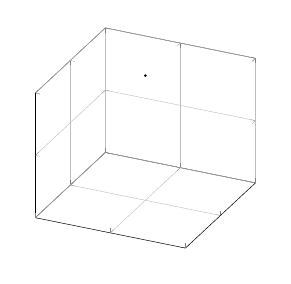
\begin{tikzpicture}[scale=0.4]
        \begin{axis}[width=0.707\textwidth, height=0.707\textwidth,xmax=1, xmin=-1, ymax=1, ymin=-1, zmax=1, zmin=-1, grid=major, xtick={-1,0,1}, xticklabels={,,}, ytick={-1,0,1}, yticklabels={,,}, ztick={-1,0,1}, zticklabels={,,}]
          \addplot3+[only marks, mark options={scale=0.5}, black] coordinates {(0,0,1)};
        \end{axis}
    \end{tikzpicture}}
   \vcenteredhbox{\begin{tikzpicture}[scale=0.4]
        \begin{polaraxis}[width=\textwidth, ymin=0, ymax=1, ytick={0,0.5,1}, yticklabels={1,0.5,0}, ytick={0,0.5,1}, yticklabels={0,45,90}, ylabel={Polar angle [$^{\circ}$]}, , xlabel={Azimuth angle [$^{\circ}$]}]
            \addplot+[only marks, mark options={scale=0.7}, data cs=cart, black] coordinates {(0,0)};
    	\end{polaraxis}
    \end{tikzpicture}}\\
    $\kappa\rightarrow\infty$
\end{minipage}\vspace{2ex}  \caption{Visualisation of 1000 sample directions drawn from Von-Mises-Fisher distribution with varying $\kappa$. Left half of each figure shows the 3-d scatter plot, right half shows a polar plot of the sampled directions for each value of $\kappa$.}
  }
  \label{fig:chapter7 exp1 VanMises draw}
 \end{figure}

\subsection{Feasibility study on fixed monkey spinal cord}
Scans were performed on an experimental 4.7 Tesla scanner (Varian Inc., Palo Alto, CA, USA) in collaboration with the Danish Research Centre for Magnetic Resonance (DRCMR). To make best use of the hardware, we carry out the protocol optimisation as described above but increase $|G|_{max}$ to $300mT/m$. We also adjust for differences in tissue properties between live and fixed tissue, e.g. decreased diffusivity and shrinkage of axon diameters, based on preliminary DTI analysis of the tissue sample (see modified tissue parameters in Table~\ref{tab: chapter7 exp1 model opt parameters ex-vivo}). Scan time in this experiment was limited to 12h only. To retain acceptable image resolution and SNR within the given time frame, we reduced the number of acquisitions to $M=4$ and $N=30$. Furthermore, we only had time to test the {\FD} protocol in this experiment. The resulting protocol is summarised in Table~\ref{XX} and described more comprehensively in Appendix \ref{app:chapter7 protocols 300mT}. 
\paragraph{}
We used a volume coil for transmission and a homemade 20 mm surface coil was used as receive coil. The data was was acquired using a spin-echo sequence with single line readout and a conventional pulsed gradient spin-echo preparation \citep{Stejskal:1965}.  TE/TR were 59/2000 ms, field of view (FoV) was $10\times 10 mm^2$. The matrix size was 64x64 and was 2-D interpolated to 128x128 leading to an axial in-plane resolution of $79 \times 79 \mu m^2$. To support the high in-plane resolution we acquire thick slices of 1.5mm to achieve acceptable \gls{SNR} in our data. The protocol was repeated 4 times with a total imaging time of 13 h. The magnitude images of the four repeated measurements were averaged offline prior to analysis.

\begin{table}[!ht]
	\caption{Adjusted ex-vivo tissue model parameters used for pre-clinical scan optimisation (changes to in-vivo protocol are displayed in red).}
    \centering
    \vspace{2ex}	
    % Cylinder
    \begin{tabular}{y{0.1\textwidth}y{0.25\textwidth}}
    \addlinespace
    \toprule
    \multicolumn{2}{c}{\textbf{Cylinder}} \\
    \multicolumn{2}{c}{(intra-axonal)} \\
    \midrule
    $f_{intra}$ & $0.7$ \\
    $D_{\|}$ & {\color{red}$4\cdot 10^{-10}$ $s/mm^2$} \\
    $D_{\bot} $ & {\color{red}$2.5\cdot 10^{-10}$ $s/mm^2$} \\
    dir   & $[0,0,1]^T$ \\
    R & {\color{red}$\{0.5,1,2\}\mu m$} \\
    \bottomrule
    \end{tabular}%
    \hspace{0.15\textwidth}
    %%% Zeppelin
    \begin{tabular}{y{0.1\textwidth}y{0.25\textwidth}}
    \addlinespace
    \toprule
    \multicolumn{2}{c}{\textbf{Axially symmetric tensor}} \\
    \multicolumn{2}{c}{(extra-axonal)} \\
    \midrule
    $f_{extra}$& $0.3$ \\
    $D_{\parallel}$ & {\color{red}$4\cdot 10^{-10}$ $m^2/s$} \\
    $D_{\bot} $ & {\color{red}$2.5\cdot 10^{-10}$ $s/m^2/s$} \\
    dir & $[0,0,1]^T$ \\
    \bottomrule
    & \\ %empty line to level tables
    \end{tabular}%
    \label{tab: chapter7 exp1 model opt parameters ex-vivo}
    \vspace{2ex}	
\end{table}

\subsection{Model fitting}
A voxel-wise fit of the MR signal is performed using a fitting method similar to \citep{Alexander:2010}. We define the objective function as the maximum likelihood of model parameters given the observed MR signals under Rician noise ($\sigma=0.05$). We use the multi-run fitting routine of \citep{Panagiotaki:2012} to find an initial parameters, which determines the best parameter estimates from multiple gradient-descend runs with pertubed starting points (n=20 in our case). Based on the initial parameter estimates, we then perform a \gls{MCMC} algorithm to determine the posterior distributions of the model parameters. To ensure convergence, we used the following, rather conservative setting for the \gls{MCMC} algorithm: burn-in of 5000, sample interval of 1000, 5\% parameter pertubations with uniform, uninformative priors.

To increase stability of the fitting we fix $D_\parallel$ to its true value of $1.7mm/s^2$ similar to previous studies \citep{Assaf:2008,Barazany:2009,Alexander:2010}. Moreover, $D_\bot$ is approximated by the tortuosity formulation of \citep{Szafer:1995}:
$$
    D_{\bot} = f_{intra}\cdot D_{\parallel}.
$$


For {\DO} and {\FD}, we also found our method to be very unstable with respect to determining the correct principal diffusion direction of the model, even when the fibre direction was close to $[0,0,1]^T$. This likely stems from the fact that the initial guess of the direction is computed from the \gls{DT} model. While this method works fine for \OI and \SD protocols, it fails when using the optimised gradient direction sets of \DO and \FD. We therefore fix the principal fibre direction to $[0,0,1]^T$ in all experiments, unless stated otherwise.

\subsubsection*{Fixed tissue}
We chose to scan a sample of fixed monkey cervical spinal cord to test our protocol in a real biological system. The details of the sample preparation are described in \citep{Lundell:2011}. For the fixed tissue we use a slightly modified fitting routine to account for the differences between fixed and live tissue. Here we fix $D_{par}$ to $0.45\mu m/mm^2$. The volume fraction of the restricted compartment f was constrained to be in the range of $[0.5, 1.0]$. We then In each voxel, the mean of the posterior distribution of $R$ and $f_{intra}$ are calculated. For consistency with indices derived from histological examination and also previous imaging studies e.g. \citep{Alexander:2010}, maps of the axon diameter index $D=2\cdot R$ and the axonal density index $\rho=f_{intra}/\pi/R^2$ are reported.

\FloatBarrier

\section{Results}
\subsection{Accuracy and precision of parameter estimates}
Figure~\ref{fig:chapter7 exp1 boxplots 60mT} shows box plots of the fitted volume fraction $f_{intra}$ and $R$ for different cylinder radii.

definition
\begin{figure}[H]
	\centering
	\begin{tikzpicture}
	\begin{axis}[xmin=0,xmax=5,ymin=0, ymax=1,
		xtick={1,2,3,4,5},xticklabels={$1\mu m$,$2\mu m$,$5\mu m$,$10\mu m$},
        width=0.7\textwidth, height=0.5\textwidth, legend columns=6, legend style={at={(0,1.05)}, anchor=south west}, xlabel={True cylinder radius}, ylabel={Volume fraction}]

		%#1: center, #2: median, #3: 1/4 quartile, #4: 3/4 quartile, #5: -1.5IQ, #6: +1.5IQ
		\boxplot{3.70}{0.709}{0.653}{0.761}{0.579}{0.812}{red}
		\boxplot{3.90}{0.738}{0.684}{0.787}{0.616}{0.841}{green}
		\boxplot{4.10}{0.689}{0.656}{0.719}{0.619}{0.761}{blue}
		\boxplot{4.30}{0.724}{0.673}{0.764}{0.623}{0.803}{cyan}


        \addlegendentry{\OI}
        \addlegendentry{\SD}
        \addlegendentry{\DO}
        \addlegendentry{\FD}



        \addplot[black, dashed] coordinates{(0.5,0.7) (1.5,0.7)};
        \addlegendentry{ground truth};

		\boxplot{0.70}{0.700}{0.694}{0.707}{0.688}{0.716}{red}
		\boxplot{1.70}{0.692}{0.685}{0.699}{0.678}{0.715}{red}
		\boxplot{2.70}{0.700}{0.687}{0.714}{0.672}{0.731}{red}
		\boxplot{0.90}{0.698}{0.692}{0.703}{0.686}{0.709}{green}
		\boxplot{1.90}{0.705}{0.698}{0.711}{0.691}{0.725}{green}
		\boxplot{2.90}{0.712}{0.699}{0.726}{0.682}{0.743}{green}
		\boxplot{1.10}{0.703}{0.699}{0.706}{0.695}{0.712}{blue}
		\boxplot{2.10}{0.697}{0.693}{0.701}{0.688}{0.711}{blue}
		\boxplot{3.10}{0.698}{0.691}{0.705}{0.683}{0.713}{blue}
		\boxplot{1.30}{0.703}{0.701}{0.706}{0.697}{0.709}{cyan}
		\boxplot{2.30}{0.703}{0.699}{0.710}{0.693}{0.721}{cyan}
		\boxplot{3.30}{0.714}{0.708}{0.721}{0.699}{0.730}{cyan}


        \addplot+[only marks, mark=text, text mark={*}, mark options={scale=0.7},red!30] table[x index=0,y index=1] {chapter7/figs/OInv_60mT_outliers_f.dat};
        \addplot+[only marks, mark=text, text mark={*}, mark options={scale=0.7},green!30] table[x index=0,y index=1] {chapter7/figs/OI_60mT_outliers_f.dat};
        \addplot+[only marks, mark=text, text mark={*}, mark options={scale=0.7},blue!30] table[x index=0,y index=1] {chapter7/figs/DO_60mT_outliers_f.dat};
        \addplot+[only marks, mark=text, text mark={*}, mark options={scale=0.7},cyan!30] table[x index=0,y index=1] {chapter7/figs/FD_60mT_outliers_f.dat};


        \addplot[black, dashed] coordinates{(0.5,0.7) (1.5,0.7)};
        \addplot[black, dashed] coordinates{(1.5,0.7) (2.5,0.7)};
        \addplot[black, dashed] coordinates{(2.5,0.7) (3.5,0.7)};
        \addplot[black, dashed] coordinates{(3.5,0.7) (4.5,0.7)};


	\end{axis}
\end{tikzpicture}

	\begin{tikzpicture}
	\begin{axis}[xmin=0,xmax=5,ymin=0, ymax=15,
		xtick={1,2,3,4,5},xticklabels={$1\mu m$,$2\mu m$,$5\mu m$,$10\mu m$},
        width=0.7\textwidth, height=0.5\textwidth, xlabel={True cylinder radius}, ylabel={Fitted radius $[\mu m]$}]

		\boxplot{3.70}{10.126}{9.657}{10.462}{8.736}{10.725}{red}
		\boxplot{3.90}{10.186}{9.810}{10.455}{9.088}{10.662}{green}
		\boxplot{4.10}{9.941}{9.640}{10.190}{9.244}{10.471}{blue}
		\boxplot{4.30}{10.141}{9.767}{10.396}{9.300}{10.611}{cyan}
		

		%#1: center, #2: median, #3: 1/4 quartile, #4: 3/4 quartile, #5: -1.5IQ, #6: +1.5IQ

        %\addlegendentry{OInv};
        %\addlegendentry{OI};
        %\addlegendentry{DO};
        %\addlegendentry{FD};

		\boxplot{0.70}{1.326}{0.705}{2.087}{0.233}{2.802}{red}
		\boxplot{1.70}{1.704}{0.884}{2.534}{0.244}{3.237}{red}
		\boxplot{2.70}{4.996}{4.841}{5.151}{4.603}{5.359}{red}
		\boxplot{0.90}{0.577}{0.284}{0.871}{0.132}{1.216}{green}
		\boxplot{1.90}{1.567}{0.895}{2.348}{0.261}{3.111}{green}
		\boxplot{2.90}{5.107}{4.952}{5.259}{4.733}{5.442}{green}
		\boxplot{1.10}{1.103}{0.558}{1.743}{0.192}{2.494}{blue}
		\boxplot{2.10}{1.674}{0.903}{2.328}{0.281}{2.828}{blue}
		\boxplot{3.10}{5.006}{4.932}{5.077}{4.829}{5.162}{blue}
		\boxplot{1.30}{0.349}{0.201}{0.467}{0.117}{0.572}{cyan}
		\boxplot{2.30}{2.026}{1.109}{2.593}{0.345}{3.033}{cyan}
		\boxplot{3.30}{5.097}{5.033}{5.171}{4.952}{5.253}{cyan}








        \addplot+[only marks, mark=text, text mark={*}, mark options={scale=0.5},draw opacity=50] table[x index=0,y index=1] {chapter7/figs/OInv_60mT_outliers.dat};
        \addplot+[ only marks, mark=text, text mark={*}, mark options={scale=0.5},green, draw opacity=50] table[x index=0,y index=1] {chapter7/figs/OI_60mT_outliers.dat};
        \addplot+[ only marks, mark=text, text mark={*}, mark options={scale=0.5},blue, draw opacity=50] table[x index=0,y index=1] {chapter7/figs/DO_60mT_outliers.dat};
        \addplot+[ only marks, mark=text, text mark={*}, mark options={scale=0.5},cyan, draw opacity=50] table[x index=0,y index=1] {chapter7/figs/FD_60mT_outliers.dat};


        \addplot[black, dashed] coordinates{(0.5,1) (1.5,1)};
        \addplot[black, dashed] coordinates{(1.5,2) (2.5,2)};
        \addplot[black, dashed] coordinates{(2.5,5) (3.5,5)};
        \addplot[black, dashed] coordinates{(3.5,10) (4.5,10)};

	\end{axis}
\end{tikzpicture}

	\caption{Boxplots of estimated $f_{intra}$ and $R$ for different cylinder radii.}
	\label{fig:chapter7 exp1 boxplots 60mT}
\end{figure}


\paragraph{} All protocols can successfully recover the correct value for $f_{intra}$ for all radii 1, 2 and 5 $\mu m$ with the posterior distributions being centred around the true value $f_{intra}=0.7$ with little variance. $R=10\mu m$ significantly more variance in the estimates is observed for in all protocols. Further we find also find the estimates to be less accurate, mainly in {\SF} and {\SD}, which overestimate of $f_{intra}$ slightly.

\begin{figure}[H]
	 \centering
	 \begin{tikzpicture}[scale=0.7]
	\begin{axis}[
			xmin=0,
			xmax=15,
			ymin=0,
			ymax=700,
            title={\OI},
            width=0.7*\textwidth,
            height=0.4*\textwidth,
            area legend,
            legend style={font=\footnotesize},
		]
		\addplot[const plot, fill=red!70!green,fill opacity=0.8] table[x index=0,y index=2] {chapter7/figs/hist_OInv60mT_1_2_5_10.dat} \closedcycle;
		\addplot[const plot, fill=red!70!blue,fill opacity=0.8] table[x index=0,y index=3] {chapter7/figs/hist_OInv60mT_1_2_5_10.dat} \closedcycle;
		\addplot[const plot, fill=red!70!black,fill opacity=0.5] table[x index=0,y index=4] {chapter7/figs/hist_OInv60mT_1_2_5_10.dat} \closedcycle;
		\addplot[const plot, fill=red!70!yellow, fill opacity=0.5] table[x index=0,y index=1] {chapter7/figs/hist_OInv60mT_1_2_5_10.dat} \closedcycle;
		\addplot[dashed, black, line legend] coordinates {(1,0) (1,1000)};
		\addplot[dashed, black] coordinates {(2,0) (2,1000)};
		\addplot[dashed, black] coordinates {(5,0) (5,1000)};
		\addplot[dashed, black] coordinates {(10,0) (10,1000)};
		\legend{$1\mu m$,$2\mu m$,$5\mu m$,$10\mu m$};
		\end{axis}
\end{tikzpicture}
\begin{tikzpicture}[scale=0.7]
	\begin{axis}[
			xmin=0,
			xmax=15,
			ymin=0,
			ymax=700,
            title={\SD},
            width=0.7*\textwidth,
            height=0.4*\textwidth,
            area legend
		]
		\addplot[const plot, fill=green!70!green,fill opacity=0.8] table[x index=0,y index=2] {chapter7/figs/hist_OI60mT_1_2_5_10.dat} \closedcycle;
		\addplot[const plot, fill=green!70!blue,fill opacity=0.8] table[x index=0,y index=3] {chapter7/figs/hist_OI60mT_1_2_5_10.dat} \closedcycle;
		\addplot[const plot, fill=green!70!black,fill opacity=0.5] table[x index=0,y index=4] {chapter7/figs/hist_OI60mT_1_2_5_10.dat} \closedcycle;
		\addplot[const plot, fill=green!70!yellow, fill opacity=0.5] table[x index=0,y index=1] {chapter7/figs/hist_OI60mT_1_2_5_10.dat} \closedcycle;
		\addplot[line legend, dashed, black] coordinates {(1,0) (1,1000)};
		\addplot[dashed, black] coordinates {(2,0) (2,1000)};
		\addplot[dashed, black] coordinates {(5,0) (5,1000)};
		\addplot[dashed, black] coordinates {(10,0) (10,1000)};
		\legend{$1\mu m$,$2\mu m$,$5\mu m$,$10\mu m$};
		\end{axis}
\end{tikzpicture}
\begin{tikzpicture}[scale=0.7]
	\begin{axis}[
			xmin=0,
			xmax=15,
			ymin=0,
			ymax=700,
            title={\DO},
            width=0.7*\textwidth,
            height=0.4*\textwidth,
            area legend
		]
		\addplot[const plot, fill=blue!60!green,fill opacity=0.8] table[x index=0,y index=2] {chapter7/figs/hist_DO60mT_1_2_5_10.dat} \closedcycle;
		\addplot[const plot, fill=blue!60!blue,fill opacity=0.8] table[x index=0,y index=3] {chapter7/figs/hist_DO60mT_1_2_5_10.dat} \closedcycle;
		\addplot[const plot, fill=blue!60!black,fill opacity=0.5] table[x index=0,y index=4] {chapter7/figs/hist_DO60mT_1_2_5_10.dat} \closedcycle;		
		\addplot[const plot, fill=blue!60!yellow, fill opacity=0.5] table[x index=0,y index=1] {chapter7/figs/hist_DO60mT_1_2_5_10.dat} \closedcycle;
		\addplot[line legend, dashed, black] coordinates {(1,0) (1,1000)};
		\addplot[dashed, black] coordinates {(2,0) (2,1000)};
		\addplot[dashed, black] coordinates {(5,0) (5,1000)};
		\addplot[dashed, black] coordinates {(10,0) (10,1000)};
		\legend{$1\mu m$,$2\mu m$,$5\mu m$,$10\mu m$};
		\end{axis}
\end{tikzpicture}
\begin{tikzpicture}[scale=0.7]
	\begin{axis}[
			xmin=0,
			xmax=15,
			ymin=0,
			ymax=700,
            title={\FD},
            width=0.7*\textwidth,
            height=0.4*\textwidth,
            area legend
		]
		\addplot[const plot, fill=cyan!60!green,fill opacity=0.8] table[x index=0,y index=2] {chapter7/figs/hist_FD60mT_1_2_5_10.dat} \closedcycle;
		\addplot[const plot, fill=cyan!60!blue,fill opacity=0.8] table[x index=0,y index=3] {chapter7/figs/hist_FD60mT_1_2_5_10.dat} \closedcycle;
		\addplot[const plot, fill=cyan!60!black,fill opacity=0.5] table[x index=0,y index=4] {chapter7/figs/hist_FD60mT_1_2_5_10.dat} \closedcycle;		
		\addplot[const plot, fill=cyan!60!yellow, fill opacity=0.5] table[x index=0,y index=1] {chapter7/figs/hist_FD60mT_1_2_5_10.dat} \closedcycle;
		\addplot[dashed, black, line legend] coordinates {(1,0) (1,1000)};
		\addplot[dashed, black] coordinates {(2,0) (2,1000)};
		\addplot[dashed, black] coordinates {(5,0) (5,1000)};
		\addplot[dashed, black] coordinates {(10,0) (10,1000)};
		\legend{$1\mu m$,$2\mu m$,$5\mu m$,$10\mu m$};
		\end{axis}
\end{tikzpicture}

	 \caption{Histograms of fitted cylinder radius $R$ for different protocols.}
	 \label{fig:chapter7 exp1 histograms 60mT}
\end{figure}

\paragraph{} Compared to $f_{intra}$ results, we observe more variance in the posterior distributions of $R$ estimates for all protocols. Over all $R$ {\DO} and {\FD} appear to achieve better results than {\OI} and {\SD} protocols. To illustrate this better, Figure~\ref{fig:chapter7 exp1 histograms 60mT} shows the posterior distributions of $R$ for each protocol in more detail.

All protocols perform the best for $R=5\mu m$ with tight posterior distributions centred around the ground truth. While generally all protocols show very good accuracy in estimating $R$, {\DO} and {\FD} have the advantage in terms of precision as their distributions are considerably tighter than for {\OI} and {\SD}. Compared to $R=5\mu m$, $R=10\mu m$ estimates generally are broader and with a notiable  negative skew, particularily for {\OI} and {\SD} protocols.  As for $5\mu m$, {\DO} and {\FD} produce more sharp parameter distributions than {\OI} and {\SD}, although the difference is less obvious. The broader distributions for $R=10\mu m$ might be explained by the long diffusion, which are necessary to estimate large radii accurately.  We assume a typical T2 signal decay of 70ms in this experiment. As shown in \citep{Alexander:STEAM}, in this regime long diffusion times can not be reached with acceptable SNR. As a consequence, for $R=10\u m$ a greater proportion of the signal will appear unrestricted and causes the underestimation of $f_{intra}$ and larger variation in radius estimates in our results.

Smaller radii $R=1\mu m$ and $R=2\mu m $ less well distinguished from each other in all protocols, with posterior distributions showing significant overlap as expected from limited gradient strength used in this experiment \citep{Alexander:2008,Alexander:2010,Siow:2012}. For small radii the \gls{COM} effect on small radii prohibits any contrast between different $R$, which we find reflected in our posterior distributions (see Chapter~\ref{TODO} for a detailed explanation). However, {\FD} suffers least from this and clearly outperforms the other protocols as it allows much better distinction between the small radii.


\subsection{Variation of fibre direction}
Figure~\ref{fig:chapter7 exp1 angular vals 60mT} shows the root mean squared error for both $f_{intra}$ and $R$ parameters with respect to the principle orientation of diffusion for cylinders with small radius $R=2\mu m$ and large radius $R=5\mu m$. As in the previous experiment, all the protocols generally perform better for $R=5\mu m$ than $R=2\mu m$. Therefore, the most marked differences between protocols appear in the $R=2\mu m$ dataset.
\paragraph{}
The plots clearly show that estimates of $f_{intra}$ are unaffected by the true diffusion orientation in all protocols for $R=2\mu m$. While this expected for {\OI} and {\SD}, we can explain the performance of {\FD} and {\DO} explained by the small cylinder radius, which allows {\FD} and {\OI} to distinguish hindered and restricted diffusion even when the gradient scheme is not aligned perpendicular to the intra-axonal compartment. Results for $R=5\mu m$ show that $f_{intra}$ estimates are affected more by the misalignment of the gradient scheme with larger radii, although the estimation error still remains low over all different directions.

\paragraph{}
Bigger differences between the protocols can be seen in the $R$ estimation error. Again, {\OI} and {\SD} are consistent over the whole range of simulated fibre directions, with no apparent directional pattern of the estimation error. In contrast, {\FD} and {\DO} performance is considerably more impeded for larger misalignment of gradient scheme and cylinder orientation. The maximum estimation error is observed for rotation angles around $45^\circ$. With $\phi$ close to $90^\circ$, the {\SF} and {\DO} gradient direction scheme now features more measurements perpendicular and parallel to the cylinder compartment, which reduces again the fitting error. For smaller misalignments of $\phi<15^\circ$ both {\FD}/{\DO} perform very similar to the {\OI}/{\SD} protocols.

\begin{figure}[!h]
%  \ifdraft
%  {
%  	\draftpic
%  }
   {
\centering
	\subfloat[Cylinder radius $R=2\mu m$]
    {
        \begin{minipage}{\textwidth}    
        	\pgfimage[width=0.9\textwidth]{chapter7/figs/errs_2D_f_60mT.pdf}\\
            \pgfimage[width=0.9\textwidth]{chapter7/figs/errs_2D_R_60mT.pdf}
        \end{minipage}
    }
    
    
    
    \subfloat[Cylinder radius $R=5\mu m$]
    {
        \begin{minipage}{\textwidth}    
            \pgfimage[width=0.9\textwidth]{chapter7/figs/errs_2D_f_60mTR5.pdf}\\
            \pgfimage[width=0.9\textwidth]{chapter7/figs/errs_2D_R_60mTR5.pdf}
        \end{minipage}
    }
  }
	\caption{Root mean square error of $f_{intra}$ and $R$ estimates for different principle diffusion directions.}
	\label{fig:chapter7 exp1 angular vals 60mT}
\end{figure}


\paragraph{Effect of fibre dispersion: } Figure~\ref{fig:chapter7 exp1 dispersion 60mT} shows the fitted $f_{intra}$ and $R$ estimates different degrees of intra-voxel dispersion of fibre orientations. For small $\kappa$, i.e. high degrees of dispersion, we observe large errors in estimates of both $f_{intra}$ and $R$, as expected e.g. from \citep{Zhang:2011}. However, for $\kappa \ge 64$, the fitted parameters converge to their respective ground truth, despite a considerable degree of dispersion still present in those datasets. With increasing $\kappa$, there appears to be no noticable difference between the four protocols.

%\tikzset{external/export=false}
\begin{figure}[ht]
	\centering
	\begin{tikzpicture}[scale=0.7]
    \begin{axis}[xmin=0,xmax=12,ymin=0, ymax=1,
		xtick={1,2,3,4,5,6,7,8,9,10,11},xticklabels={1,2,4,8,16,32,64,128,256,512,$\infty$},
        width=0.7\textwidth, height=0.5\textwidth, legend columns=3, legend style={at={(0.05,0.05)}, anchor=south west}, xlabel={$\kappa$}, ylabel={Volume fraction}]
        \addplot+[red, mark options={fill=red}] plot[error bars/.cd, y dir=both, y explicit] table[x index=8, y index=0, y error index=1] {chapter7/figs/BW_Dispersion_f_300mT.dat};
        \addplot+[green, mark options={fill=green}] plot[error bars/.cd, y dir=both, y explicit] table[x index=8, y index=2, y error index=3] {chapter7/figs/BW_Dispersion_f_300mT.dat};
        \addplot+[blue, mark options={fill=blue}] plot[error bars/.cd, y dir=both, y explicit] table[x index=8, y index=4, y error index=5] {chapter7/figs/BW_Dispersion_f_300mT.dat};
        \addplot+[cyan, mark options={fill=cyan}] plot[error bars/.cd, y dir=both, y explicit] table[x index=8, y index=6, y error index=7] {chapter7/figs/BW_Dispersion_f_300mT.dat};
        \addplot[black, dashed] coordinates{(0.5,0.7) (11.5,0.7)};
        \legend{\OI, {\SD}, {\DO}, {\FD}, ground truth};
	\end{axis}
\end{tikzpicture}

	\begin{tikzpicture}[scale=0.7]
	\begin{axis}[xmin=0,xmax=12,ymin=0, ymax=12,
		xtick={1,2,3,4,5,6,7,8,9,10,11},xticklabels={1,2,4,8,16,32,64,128,256,512,$\infty$},
        width=0.7\textwidth, height=0.5\textwidth, legend columns=6, legend style={at={(0,1.05)}, anchor=south west}, xlabel={$\kappa$}, ylabel={Cylinder radius $[\mu m]$}]
               \addplot+[red, mark options={fill=red}] plot[error bars/.cd, y dir=both, y explicit] table[x index=8, y index=0, y error index=1] {chapter7/figs/BW_Dispersion_R_300mT.dat};
        \addplot+[green, mark options={fill=green}] plot[error bars/.cd, y dir=both, y explicit] table[x index=8, y index=2, y error index=3] {chapter7/figs/BW_Dispersion_R_300mT.dat};
        \addplot+[blue, mark options={fill=blue}] plot[error bars/.cd, y dir=both, y explicit] table[x index=8, y index=4, y error index=5] {chapter7/figs/BW_Dispersion_R_300mT.dat};
        \addplot+[cyan, mark options={fill=cyan}] plot[error bars/.cd, y dir=both, y explicit] table[x index=8, y index=6, y error index=7] {chapter7/figs/BW_Dispersion_R_300mT.dat};
        \addplot[black, dashed] coordinates{(0.5,5) (11.5,5)};        
	\end{axis}
\end{tikzpicture}

	\caption{Mean and standard deviation of posterior distribution for fitted volume fraction and radius for different $\kappa$ values.}
	\label{fig:chapter7 exp1 dispersion 60mT}
\end{figure}
%\tikzset{external/export=false}

\subsection{Proof-of-concept implementation}
Figure~\ref{fig:chapter7 exp1 monkey data} presents maps of axon diameter $D$ and axonal density $\rho$ in the upper cervical spinal cord obtained from the {\FD} protocol. We can discriminate well differences in axon diameter and axonal density indices between anatomically different white matter tracts. Dorsal and lateral sensory tracts show small axons diameters between 1--4$\mu m$ and a density of 0.03--0.08$\mu m^{-2}$. The smallest axon calibers (<1.5$\mu m$) are observed in the dorsal columns (DC) while mean axon size in the anterolateral column (ALC) is 1.5--2.5$\mu m$. The largest axons (3--4$\mu m$) are found in the corticospinal tracts (CST) together with low density of 0.01--0.02$\mu m^{-2}$. Overall, we clearly observe left-right symmetry of axon diameter and density in all tracts, which corresponds well with the known anatomical organisation of the the SC. Parameters are also consistent along the SC within the limits of anatomical variation and are in the range of values reported in previous histological evaluation of the cord \citep{GrafvonKeyserlingk:1984,Golabchi:2010}. 

\begin{figure}[ht]
	\centering
	\subfloat[Axon diameter index $D$]
	{
   	  \ifdraft
	  {
	  	\draftpic
	  }
      {
		\pgfimage[width=4cm]{chapter7/figs/monkeySC_diam.png}
      }   
	}
	\hspace{2cm}
	\subfloat[Axon density index $\rho$]
	{
      \ifdraft
	  {
	  	\draftpic
	  }
      {
		\pgfimage[width=4cm]{chapter7/figs/monkeySC_dens.png}
      }
	}
	\caption{Axial slice of upper cervical cord showing maps of $D$ and $\rho$. White markers show the approximate location of the corticospinal tracts (CST), anterolateral column (ALC) and dorsal column (DC)}
	\label{fig:chapter7 exp1 monkey data}
\end{figure}

\section{Discussion}
We presented here a novel method that provides optimal diffusion weightings and gradient directions for estimating of axonal diameter by exploiting the single fibre orientation of structures like the corpus callosum or spinal cord. We demonstrated that the {\SF} approach reduces the required amount of data by 60--75\%, while achieving similar performance to {\OI}. This translates into a considerable reduction in scan time from >1h for {\OI} to less than 20-25 minutes, which makes routine clinical implementation much more viable.  

\paragraph{}
Our results suggest that a dedicated optimisation of gradient directions is clearly beneficial over the orientation invariant \OI{} approach, both in terms of CRLB and simulated noisy data when the fibre direction is known a-priori. We find that the optimisation routine deliberately diminishes angular resolution in favour of measuring diffusion only in the most informative directions (predominantly parallel and perpendicular to the WM tracts). We noticed that our optimised gradient scheme pick out predominantly gradient directions parallel and perpendicular to the cylinder compartment, presumably to maximise sensitivity to restricted diffusion. In that respect our automatically optimised gradient schemes agree with other many other studies e.g. \citep{Stanisz:1997,Avram:2008,Assaf:2008,Panagiotaki:2012}, which only chose parallel and perdendicular measurements to maximise sensitive to restricted diffusion. Our results confirm that these directions give the most information about the tissue, and one should focus on those directions when the fibre configuration is known \textit{a-priori}. 


We furthermore observe that our {\FD} protocols contain slightly stronger diffusion weighting factors compared to the other protocols. We can attribute this to the custom gradient scheme, which translates to more measurements in the perpendicular direction and hence profits more from stronger diffusion attenuation than {\OI}. The simulation results show the combination of stronger diffusion weighting and custom gradient scheme is superior in estimating the cylinder radius, especially when $R$ is very small.

\paragraph{}
Considering the few number of distinct gradient directions, it comes to no surprise that we found the optimised gradient schemes in {\FD} and {\DO} more prone to error when the true fibre orientation differs from the one assumed in the optimisation process. However, when the misalignment was less than 15$^\circ$ (as expected in coherent WM structures) the impact was neglible. We are confident that with careful positioning, the {\SF} gradient scheme can be aligned to the dominant fibre directions in CC and SC with little error without diminishing the performance of the {\SF} protocols.
\paragraph{}
Finally, the feasibility study on our post-mortem SC sample demonstrates that we can estimate a reasonable range of axon diameters and densities under realistic imaging conditions, while retaining a high image resolution. Furthermore we were able to distinguish different WM tracts of the SC by both axon diameter and axon density.
\paragraph{}
There are some limiting factors to our study. Firstly, we only optimise and fit a very simple tissue model, which only allows a crude approximation of the real tissue properties. Other, more complex, models might be a better representation of the real tissue microstructure, e.g. modelling explicitly a distribution of axon radii \citep{Barazany:2009} or including more extra-axonal tissue compartments \citep{Stanisz:1997,Wang:2011,Panagiotaki:2012}.  While these models might arguably be more accurate, they also require many more acquisitions and therefore do not agree with the aim of this study to reduce the scan time to less than 30 minutes. The choice of a simpler model offers a compromise of manageable data requirements and informative model parameters.
\paragraph{}
Secondly, the spinal cord sample we used in this study was not available for histological processing. Despite the lack of independent validation, the differences between WM tracts agree with previous results in \citep{Golabchi:2010}. It should be noted that our results were obtained with a significantly smaller number of diffusion weighted directions and b-factors compared to other studies \citep{Assaf:2008,Barazany:2009,Panagiotaki:2012}, making it more comparable to conditions found in in-vivo scanning. Nevertheless, in many this pre-clinical setup here has many advantages over the in-vivo situation, as it profits from long scan times, high SNR and an absence of motion artefacts. Although the findings in this experiment might therefore not be directly transferable to clinical practise, the results are encouraging enough to pursue the \SF{} approach in clinical practise. In the next two chapters we will therefore focus on moving the \SF{} approach to towards a feasible in-vivo implementation on standard clinical hardware.



\FloatBarrier
\begin{subappendices}

\section{Protocols}
%\tikzset{external/export=false}
\ifdraft
{
   Appendix here
}
{
    \subsection{Protocols optimised for $|G|_{max}$=60mT/m, N=90, M=8}
    \label{app:chapter7 protocols 60mT}
    \begin{figure}
    	[H] \centering 
%%% protocol m=1 start
\begin{tikzpicture}
\node [protocolbox] (box){
   \begin{minipage}{0.45\textwidth}
   \vspace{1ex}
        \centering
        \raisebox{0cm}{\sequenceNoWeights{0.018}{0.013}{0.060}{1.000}{0.071}}
        \begin{tikzpicture}[scale=0.6]
          \begin{axis}[ xlabel=$x$, ylabel=$y$, zlabel=$z$,xmax=1, xmin=-1, ymax=1, ymin=-1, zmax=1, zmin=-1, width=3.0cm, height=3.0cm, grid=major]
          \addplot3+[only marks] table {chapter7/figs/protocols_par1/SF_OInv_62mT002.txt};
        \end{axis}
        \end{tikzpicture}
        \vspace{2ex}
   \end{minipage}
};
\node[protocolheader, right=10pt] at (box.north west) {$\mathbf{m=1}$};
\node[protocoltext] at (box.south) {\footnotesize{$\delta=13 ms$, $\Delta=18 ms$, $|G|=60 mT/m$}};
\end{tikzpicture}
%%% protocol end
%
%
%
%%% protocol m=2 start
\begin{tikzpicture}
\node [protocolbox] (box){
   \begin{minipage}{0.45\textwidth}
   \vspace{1ex}
        \centering
        \raisebox{0cm}{\sequenceNoWeights{0.018}{0.013}{0.060}{1.000}{0.071}}
        \begin{tikzpicture}[scale=0.6]
          \begin{axis}[ xlabel=$x$, ylabel=$y$, zlabel=$z$,xmax=1, xmin=-1, ymax=1, ymin=-1, zmax=1, zmin=-1, width=3.0cm, height=3.0cm, grid=major]
          \addplot3+[only marks] table {chapter7/figs/protocols_par1/SF_OInv_62mT006.txt};
        \end{axis}
        \end{tikzpicture}
        \vspace{2ex}
   \end{minipage}
};
\node[protocolheader, right=10pt] at (box.north west) {$\mathbf{m=2}$};
\node[protocoltext] at (box.south) {\footnotesize{$\delta=13 ms$, $\Delta=18 ms$, $|G|=60 mT/m$}};
\end{tikzpicture}
\\[2ex]
%%% protocol end
%
%
%
%%% protocol m=3 start
\begin{tikzpicture}
\node [protocolbox] (box){
   \begin{minipage}{0.45\textwidth}
   \vspace{1ex}
        \centering
        \raisebox{0cm}{\sequenceNoWeights{0.018}{0.013}{0.060}{1.000}{0.071}}
        \begin{tikzpicture}[scale=0.6]
          \begin{axis}[ xlabel=$x$, ylabel=$y$, zlabel=$z$,xmax=1, xmin=-1, ymax=1, ymin=-1, zmax=1, zmin=-1, width=3.0cm, height=3.0cm, grid=major]
          \addplot3+[only marks] table {chapter7/figs/protocols_par1/SF_OInv_62mT004.txt};
        \end{axis}
        \end{tikzpicture}
        \vspace{2ex}
   \end{minipage}
};
\node[protocolheader, right=10pt] at (box.north west) {$\mathbf{m=3}$};
\node[protocoltext] at (box.south) {\footnotesize{$\delta=13 ms$, $\Delta=18 ms$, $|G|=60 mT/m$}};
\end{tikzpicture}
%%% protocol end
%
%
%
%%% protocol m=4 start
\begin{tikzpicture}
\node [protocolbox] (box){
   \begin{minipage}{0.45\textwidth}
   \vspace{1ex}
        \centering
        \raisebox{0cm}{\sequenceNoWeights{0.018}{0.013}{0.060}{1.000}{0.071}}
        \begin{tikzpicture}[scale=0.6]
          \begin{axis}[ xlabel=$x$, ylabel=$y$, zlabel=$z$,xmax=1, xmin=-1, ymax=1, ymin=-1, zmax=1, zmin=-1, width=3.0cm, height=3.0cm, grid=major]
          \addplot3+[only marks] table {chapter7/figs/protocols_par1/SF_OInv_62mT008.txt};
        \end{axis}
        \end{tikzpicture}
        \vspace{2ex}
   \end{minipage}
};
\node[protocolheader, right=10pt] at (box.north west) {$\mathbf{m=4}$};
\node[protocoltext] at (box.south) {\footnotesize{$\delta=13 ms$, $\Delta=18 ms$, $|G|=60 mT/m$}};
\end{tikzpicture}
\\[2ex]
%%% protocol end
%
%
%
%%% protocol m=5 start
\begin{tikzpicture}
\node [protocolbox] (box){
   \begin{minipage}{0.45\textwidth}
   \vspace{1ex}
        \centering
        \raisebox{0cm}{\sequenceNoWeights{0.048}{0.023}{0.031}{1.000}{0.071}}
        \begin{tikzpicture}[scale=0.6]
          \begin{axis}[ xlabel=$x$, ylabel=$y$, zlabel=$z$,xmax=1, xmin=-1, ymax=1, ymin=-1, zmax=1, zmin=-1, width=3.0cm, height=3.0cm, grid=major]
          \addplot3+[only marks] table {chapter7/figs/protocols_par1/SF_OInv_62mT003.txt};
        \end{axis}
        \end{tikzpicture}
        \vspace{2ex}
   \end{minipage}
};
\node[protocolheader, right=10pt] at (box.north west) {$\mathbf{m=5}$};
\node[protocoltext] at (box.south) {\footnotesize{$\delta=23 ms$, $\Delta=48 ms$, $|G|=31 mT/m$}};
\end{tikzpicture}
%%% protocol end
%
%
%
%%% protocol m=6 start
\begin{tikzpicture}
\node [protocolbox] (box){
   \begin{minipage}{0.45\textwidth}
   \vspace{1ex}
        \centering
        \raisebox{0.1cm}{\sequenceNoWeights{0.047}{0.024}{0.032}{1.000}{0.071}}
        \begin{tikzpicture}[scale=0.6]
          \begin{axis}[ xlabel=$x$, ylabel=$y$, zlabel=$z$,xmax=1, xmin=-1, ymax=1, ymin=-1, zmax=1, zmin=-1, width=3.0cm, height=3.0cm, grid=major]
          \addplot3+[only marks] table {chapter7/figs/protocols_par1/SF_OInv_62mT001.txt};
        \end{axis}
        \end{tikzpicture}
        \vspace{2ex}
   \end{minipage}
};
\node[protocolheader, right=10pt] at (box.north west) {$\mathbf{m=6}$};
\node[protocoltext] at (box.south) {\footnotesize{$\delta=24 ms$, $\Delta=47 ms$, $|G|=32 mT/m$}};
\end{tikzpicture}
\\[2ex]
%%% protocol end
%
%
%
%%% protocol m=7 start
\begin{tikzpicture}
\node [protocolbox] (box){
   \begin{minipage}{0.45\textwidth}
   \vspace{1ex}
        \centering
        \raisebox{0.1cm}{\sequenceNoWeights{0.045}{0.026}{0.039}{1.000}{0.071}}
        \begin{tikzpicture}[scale=0.6]
          \begin{axis}[ xlabel=$x$, ylabel=$y$, zlabel=$z$,xmax=1, xmin=-1, ymax=1, ymin=-1, zmax=1, zmin=-1, width=3.0cm, height=3.0cm, grid=major]
          \addplot3+[only marks] table {chapter7/figs/protocols_par1/SF_OInv_62mT005.txt};
        \end{axis}
        \end{tikzpicture}
        \vspace{2ex}
   \end{minipage}
};
\node[protocolheader, right=10pt] at (box.north west) {$\mathbf{m=7}$};
\node[protocoltext] at (box.south) {\footnotesize{$\delta=26 ms$, $\Delta=45 ms$, $|G|=39 mT/m$}};
\end{tikzpicture}
%%% protocol end
%
%
%
%%% protocol m=8 start
\begin{tikzpicture}
\node [protocolbox] (box){
   \begin{minipage}{0.45\textwidth}
   \vspace{1ex}
        \centering
        \raisebox{0.1cm}{\sequenceNoWeights{0.038}{0.033}{0.060}{1.000}{0.071}}
        \begin{tikzpicture}[scale=0.6]
          \begin{axis}[ xlabel=$x$, ylabel=$y$, zlabel=$z$,xmax=1, xmin=-1, ymax=1, ymin=-1, zmax=1, zmin=-1, width=3.0cm, height=3.0cm, grid=major]
          \addplot3+[only marks] table {chapter7/figs/protocols_par1/SF_OInv_62mT007.txt};
        \end{axis}
        \end{tikzpicture}
        \vspace{2ex}
   \end{minipage}
};
\node[protocolheader, right=10pt] at (box.north west) {$\mathbf{m=8}$};
\node[protocoltext] at (box.south) {\footnotesize{$\delta=33 ms$, $\Delta=38 ms$, $|G|=60 mT/m$}};
\end{tikzpicture}
\\[2ex]
%%% protocol end
%
%
%  \caption{\OI protocol optimised for clinical gradient strength.}
       \label{fig:chapter7 exp1 OINV_62mT}
    \end{figure}
    \begin{figure}
    	[H] \centering %%% protocol m=1 start
\begin{tikzpicture}
\node [protocolbox] (box){
   \begin{minipage}{0.45\textwidth}
   \vspace{1ex}
        \centering
        \raisebox{0.1cm}{\sequenceNoWeights{0.018}{0.013}{0.060}{1.000}{0.071}}
        \begin{tikzpicture}[scale=0.6]
          \begin{axis}[ xlabel=$x$, ylabel=$y$, zlabel=$z$,xmax=1, xmin=-1, ymax=1, ymin=-1, zmax=1, zmin=-1, width=3.0cm, height=3.0cm, grid=major]
          \addplot3+[only marks] table {chapter7/figs/protocols_par1/SF_OI_60mT004.txt};
        \end{axis}
        \end{tikzpicture}
        \vspace{2ex}
   \end{minipage}
};
\node[protocolheader, right=10pt] at (box.north west) {$\mathbf{m=1}$};
\node[protocoltext] at (box.south) {\footnotesize{$\delta=13 ms$, $\Delta=18 ms$, $|G|=60 mT/m$}};
\end{tikzpicture}
%%% protocol end
%
%
%
%%% protocol m=2 start
\begin{tikzpicture}
\node [protocolbox] (box){
   \begin{minipage}{0.45\textwidth}
   \vspace{1ex}
        \centering
        \raisebox{0.1cm}{\sequenceNoWeights{0.018}{0.013}{0.060}{1.000}{0.071}}
        \begin{tikzpicture}[scale=0.6]
          \begin{axis}[ xlabel=$x$, ylabel=$y$, zlabel=$z$,xmax=1, xmin=-1, ymax=1, ymin=-1, zmax=1, zmin=-1, width=3.0cm, height=3.0cm, grid=major]
          \addplot3+[only marks] table {chapter7/figs/protocols_par1/SF_OI_60mT007.txt};
        \end{axis}
        \end{tikzpicture}
        \vspace{2ex}
   \end{minipage}
};
\node[protocolheader, right=10pt] at (box.north west) {$\mathbf{m=2}$};
\node[protocoltext] at (box.south) {\footnotesize{$\delta=13 ms$, $\Delta=18 ms$, $|G|=60 mT/m$}};
\end{tikzpicture}
\\[2ex]
%%% protocol end
%
%
%
%%% protocol m=3 start
\begin{tikzpicture}
\node [protocolbox] (box){
   \begin{minipage}{0.45\textwidth}
   \vspace{1ex}
        \centering
        \raisebox{0.1cm}{\sequenceNoWeights{0.018}{0.013}{0.060}{1.000}{0.071}}
        \begin{tikzpicture}[scale=0.6]
          \begin{axis}[ xlabel=$x$, ylabel=$y$, zlabel=$z$,xmax=1, xmin=-1, ymax=1, ymin=-1, zmax=1, zmin=-1, width=3.0cm, height=3.0cm, grid=major]
          \addplot3+[only marks] table {chapter7/figs/protocols_par1/SF_OI_60mT003.txt};
        \end{axis}
        \end{tikzpicture}
        \vspace{2ex}
   \end{minipage}
};
\node[protocolheader, right=10pt] at (box.north west) {$\mathbf{m=3}$};
\node[protocoltext] at (box.south) {\footnotesize{$\delta=13 ms$, $\Delta=18 ms$, $|G|=60 mT/m$}};
\end{tikzpicture}
%%% protocol end
%
%
%
%%% protocol m=4 start
\begin{tikzpicture}
\node [protocolbox] (box){
   \begin{minipage}{0.45\textwidth}
   \vspace{1ex}
        \centering
        \raisebox{0.1cm}{\sequenceNoWeights{0.018}{0.013}{0.060}{1.000}{0.071}}
        \begin{tikzpicture}[scale=0.6]
          \begin{axis}[ xlabel=$x$, ylabel=$y$, zlabel=$z$,xmax=1, xmin=-1, ymax=1, ymin=-1, zmax=1, zmin=-1, width=3.0cm, height=3.0cm, grid=major]
          \addplot3+[only marks] table {chapter7/figs/protocols_par1/SF_OI_60mT008.txt};
        \end{axis}
        \end{tikzpicture}
        \vspace{2ex}
   \end{minipage}
};
\node[protocolheader, right=10pt] at (box.north west) {$\mathbf{m=4}$};
\node[protocoltext] at (box.south) {\footnotesize{$\delta=13 ms$, $\Delta=18 ms$, $|G|=60 mT/m$}};
\end{tikzpicture}
\\[2ex]
%%% protocol end
%
%
%
%%% protocol m=5 start
\begin{tikzpicture}
\node [protocolbox] (box){
   \begin{minipage}{0.45\textwidth}
   \vspace{1ex}
        \centering
        \raisebox{0.1cm}{\sequenceNoWeights{0.049}{0.022}{0.032}{1.000}{0.071}}
        \begin{tikzpicture}[scale=0.6]
          \begin{axis}[ xlabel=$x$, ylabel=$y$, zlabel=$z$,xmax=1, xmin=-1, ymax=1, ymin=-1, zmax=1, zmin=-1, width=3.0cm, height=3.0cm, grid=major]
          \addplot3+[only marks] table {chapter7/figs/protocols_par1/SF_OI_60mT006.txt};
        \end{axis}
        \end{tikzpicture}
        \vspace{2ex}
   \end{minipage}
};
\node[protocolheader, right=10pt] at (box.north west) {$\mathbf{m=5}$};
\node[protocoltext] at (box.south) {\footnotesize{$\delta=22 ms$, $\Delta=49 ms$, $|G|=32 mT/m$}};
\end{tikzpicture}
%%% protocol end
%
%
%
%%% protocol m=6 start
\begin{tikzpicture}
\node [protocolbox] (box){
   \begin{minipage}{0.45\textwidth}
   \vspace{1ex}
        \centering
        \raisebox{0.1cm}{\sequenceNoWeights{0.046}{0.025}{0.032}{1.000}{0.071}}
        \begin{tikzpicture}[scale=0.6]
          \begin{axis}[ xlabel=$x$, ylabel=$y$, zlabel=$z$,xmax=1, xmin=-1, ymax=1, ymin=-1, zmax=1, zmin=-1, width=3.0cm, height=3.0cm, grid=major]
          \addplot3+[only marks] table {chapter7/figs/protocols_par1/SF_OI_60mT001.txt};
        \end{axis}
        \end{tikzpicture}
        \vspace{2ex}
   \end{minipage}
};
\node[protocolheader, right=10pt] at (box.north west) {$\mathbf{m=6}$};
\node[protocoltext] at (box.south) {\footnotesize{$\delta=25 ms$, $\Delta=46 ms$, $|G|=32 mT/m$}};
\end{tikzpicture}
\\[2ex]
%%% protocol end
%
%
%
%%% protocol m=7 start
\begin{tikzpicture}
\node [protocolbox] (box){
   \begin{minipage}{0.45\textwidth}
   \vspace{1ex}
        \centering
        \raisebox{0.1cm}{\sequenceNoWeights{0.044}{0.026}{0.039}{1.000}{0.071}}
        \begin{tikzpicture}[scale=0.6]
          \begin{axis}[ xlabel=$x$, ylabel=$y$, zlabel=$z$,xmax=1, xmin=-1, ymax=1, ymin=-1, zmax=1, zmin=-1, width=3.0cm, height=3.0cm, grid=major]
          \addplot3+[only marks] table {chapter7/figs/protocols_par1/SF_OI_60mT002.txt};
        \end{axis}
        \end{tikzpicture}
        \vspace{2ex}
   \end{minipage}
};
\node[protocolheader, right=10pt] at (box.north west) {$\mathbf{m=7}$};
\node[protocoltext] at (box.south) {\footnotesize{$\delta=26 ms$, $\Delta=44 ms$, $|G|=39 mT/m$}};
\end{tikzpicture}
%%% protocol end
%
%
%
%%% protocol m=8 start
\begin{tikzpicture}
\node [protocolbox] (box){
   \begin{minipage}{0.45\textwidth}
   \vspace{1ex}
        \centering
        \raisebox{0.1cm}{\sequenceNoWeights{0.038}{0.033}{0.060}{1.000}{0.071}}
        \begin{tikzpicture}[scale=0.6]
          \begin{axis}[ xlabel=$x$, ylabel=$y$, zlabel=$z$,xmax=1, xmin=-1, ymax=1, ymin=-1, zmax=1, zmin=-1, width=3.0cm, height=3.0cm, grid=major]
          \addplot3+[only marks] table {chapter7/figs/protocols_par1/SF_OI_60mT005.txt};
        \end{axis}
        \end{tikzpicture}
        \vspace{2ex}
   \end{minipage}
};
\node[protocolheader, right=10pt] at (box.north west) {$\mathbf{m=8}$};
\node[protocoltext] at (box.south) {\footnotesize{$\delta=33 ms$, $\Delta=38 ms$, $|G|=60 mT/m$}};
\end{tikzpicture} \caption{\SD protocol optimised for clinical gradient strength}
       \label{fig:chapter7 exp1 SAMEDIRS_62mT}
    \end{figure}
    \begin{figure}
    	[H] \centering %%% protocol m=1 start
\begin{tikzpicture}
\node [protocolbox] (box){
   \begin{minipage}{0.45\textwidth}
   \vspace{1ex}
        \centering
        \raisebox{0.1cm}{\sequenceNoWeights{0.018}{0.013}{0.060}{1.000}{0.071}}
        \begin{tikzpicture}[scale=0.6]
          \begin{axis}[ xlabel=$x$, ylabel=$y$, zlabel=$z$,xmax=1, xmin=-1, ymax=1, ymin=-1, zmax=1, zmin=0, width=3.0cm, height=3.0cm, grid=major]
          \addplot3+[only marks] table {chapter7/figs/protocols_par1/SF_DO_60mT004.txt};
        \end{axis}
        \end{tikzpicture}
   \end{minipage}
};
\node[protocolheader, right=10pt] at (box.north west) {$\mathbf{m=1}$};
\node[protocoltext] at (box.south) {\footnotesize{$\delta=13 ms$, $\Delta=18 ms$, $|G|=60 mT/m$}};
\end{tikzpicture}
%%% protocol end
%
%
%
%%% protocol m=2 start
\begin{tikzpicture}
\node [protocolbox] (box){
   \begin{minipage}{0.45\textwidth}
   \vspace{1ex}
        \centering
        \raisebox{0.1cm}{\sequenceNoWeights{0.018}{0.013}{0.060}{1.000}{0.071}}
        \begin{tikzpicture}[scale=0.6]
          \begin{axis}[ xlabel=$x$, ylabel=$y$, zlabel=$z$,xmax=1, xmin=-1, ymax=1, ymin=-1, zmax=1, zmin=0, width=3.0cm, height=3.0cm, grid=major]
          \addplot3+[only marks] table {chapter7/figs/protocols_par1/SF_DO_60mT007.txt};
        \end{axis}
        \end{tikzpicture}
        \vspace{2ex}
   \end{minipage}
};
\node[protocolheader, right=10pt] at (box.north west) {$\mathbf{m=2}$};
\node[protocoltext] at (box.south) {\footnotesize{$\delta=13 ms$, $\Delta=18 ms$, $|G|=60 mT/m$}};
\end{tikzpicture}
\\[2ex]
%%% protocol end
%
%
%
%%% protocol m=3 start
\begin{tikzpicture}
\node [protocolbox] (box){
   \begin{minipage}{0.45\textwidth}
   \vspace{1ex}
        \centering
        \raisebox{0.1cm}{\sequenceNoWeights{0.018}{0.013}{0.060}{1.000}{0.071}}
        \begin{tikzpicture}[scale=0.6]
          \begin{axis}[ xlabel=$x$, ylabel=$y$, zlabel=$z$,xmax=1, xmin=-1, ymax=1, ymin=-1, zmax=1, zmin=0, width=3.0cm, height=3.0cm, grid=major]
          \addplot3+[only marks] table {chapter7/figs/protocols_par1/SF_DO_60mT003.txt};
        \end{axis}
        \end{tikzpicture}
        \vspace{2ex}
   \end{minipage}
};
\node[protocolheader, right=10pt] at (box.north west) {$\mathbf{m=3}$};
\node[protocoltext] at (box.south) {\footnotesize{$\delta=13 ms$, $\Delta=18 ms$, $|G|=60 mT/m$}};
\end{tikzpicture}
%%% protocol end
%
%
%
%%% protocol m=4 start
\begin{tikzpicture}
\node [protocolbox] (box){
   \begin{minipage}{0.45\textwidth}
   \vspace{1ex}
        \centering
        \raisebox{0.1cm}{\sequenceNoWeights{0.018}{0.013}{0.060}{1.000}{0.071}}
        \begin{tikzpicture}[scale=0.6]
          \begin{axis}[ xlabel=$x$, ylabel=$y$, zlabel=$z$,xmax=1, xmin=-1, ymax=1, ymin=-1, zmax=1, zmin=0, width=3.0cm, height=3.0cm, grid=major]
          \addplot3+[only marks] table {chapter7/figs/protocols_par1/SF_DO_60mT008.txt};
        \end{axis}
        \end{tikzpicture}
        \vspace{2ex}
   \end{minipage}
};
\node[protocolheader, right=10pt] at (box.north west) {$\mathbf{m=4}$};
\node[protocoltext] at (box.south) {\footnotesize{$\delta=13 ms$, $\Delta=18 ms$, $|G|=60 mT/m$}};
\end{tikzpicture}
\\[2ex]
%%% protocol end
%
%
%
%%% protocol m=5 start
\begin{tikzpicture}
\node [protocolbox] (box){
   \begin{minipage}{0.45\textwidth}
   \vspace{1ex}
        \centering
        \raisebox{0.1cm}{\sequenceNoWeights{0.049}{0.022}{0.032}{1.000}{0.071}}
        \begin{tikzpicture}[scale=0.6]
          \begin{axis}[ xlabel=$x$, ylabel=$y$, zlabel=$z$,xmax=1, xmin=-1, ymax=1, ymin=-1, zmax=1, zmin=0, width=3.0cm, height=3.0cm, grid=major]
          \addplot3+[only marks] table {chapter7/figs/protocols_par1/SF_DO_60mT006.txt};
        \end{axis}
        \end{tikzpicture}
        \vspace{2ex}
   \end{minipage}
};
\node[protocolheader, right=10pt] at (box.north west) {$\mathbf{m=5}$};
\node[protocoltext] at (box.south) {\footnotesize{$\delta=22 ms$, $\Delta=49 ms$, $|G|=32 mT/m$}};
\end{tikzpicture}
%%% protocol end
%
%
%
%%% protocol m=6 start
\begin{tikzpicture}
\node [protocolbox] (box){
   \begin{minipage}{0.45\textwidth}
   \vspace{1ex}
        \centering
        \raisebox{0.1cm}{\sequenceNoWeights{0.046}{0.025}{0.032}{1.000}{0.071}}
        \begin{tikzpicture}[scale=0.6]
          \begin{axis}[ xlabel=$x$, ylabel=$y$, zlabel=$z$,xmax=1, xmin=-1, ymax=1, ymin=-1, zmax=1, zmin=0, width=3.0cm, height=3.0cm, grid=major]
          \addplot3+[only marks] table {chapter7/figs/protocols_par1/SF_DO_60mT001.txt};
        \end{axis}
        \end{tikzpicture}
        \vspace{2ex}
   \end{minipage}
};
\node[protocolheader, right=10pt] at (box.north west) {$\mathbf{m=6}$};
\node[protocoltext] at (box.south) {\footnotesize{$\delta=25 ms$, $\Delta=46 ms$, $|G|=32 mT/m$}};
\end{tikzpicture}
\\[2ex]
%%% protocol end
%
%
%
%%% protocol m=7 start
\begin{tikzpicture}
\node [protocolbox] (box){
   \begin{minipage}{0.45\textwidth}
   \vspace{1ex}
        \centering
        \raisebox{0.1cm}{\sequenceNoWeights{0.044}{0.026}{0.039}{1.000}{0.071}}
        \begin{tikzpicture}[scale=0.6]
          \begin{axis}[ xlabel=$x$, ylabel=$y$, zlabel=$z$,xmax=1, xmin=-1, ymax=1, ymin=-1, zmax=1, zmin=0, width=3.0cm, height=3.0cm, grid=major]
          \addplot3+[only marks] table {chapter7/figs/protocols_par1/SF_DO_60mT002.txt};
        \end{axis}
        \end{tikzpicture}
        \vspace{2ex}
   \end{minipage}
};
\node[protocolheader, right=10pt] at (box.north west) {$\mathbf{m=7}$};
\node[protocoltext] at (box.south) {\footnotesize{$\delta=26 ms$, $\Delta=44 ms$, $|G|=39 mT/m$}};
\end{tikzpicture}
%%% protocol end
%
%
%
%%% protocol m=8 start
\begin{tikzpicture}
\node [protocolbox] (box){
   \begin{minipage}{0.45\textwidth}
   \vspace{1ex}
        \centering
        \raisebox{0.1cm}{\sequenceNoWeights{0.038}{0.033}{0.060}{1.000}{0.071}}
        \begin{tikzpicture}[scale=0.6]
          \begin{axis}[ xlabel=$x$, ylabel=$y$, zlabel=$z$,xmax=1, xmin=-1, ymax=1, ymin=-1, zmax=1, zmin=0, width=3.0cm, height=3.0cm, grid=major]
          \addplot3+[only marks] table {chapter7/figs/protocols_par1/SF_DO_60mT005.txt};
        \end{axis}
        \end{tikzpicture}
        \vspace{2ex}
   \end{minipage}
};
\node[protocolheader, right=10pt] at (box.north west) {$\mathbf{m=8}$};
\node[protocoltext] at (box.south) {\footnotesize{$\delta=33 ms$, $\Delta=38 ms$, $|G|=60 mT/m$}};
\end{tikzpicture}
\\[2ex]
%%% protocol end  \caption{\DO protocol optimised for clinical gradient strength}
       \label{fig:chapter7 exp1 DIRSONLY_62mT}
    \end{figure}
    \begin{figure}
    	[H] \centering %%% protocol m=1 start
\begin{tikzpicture}
\node [protocolbox] (box){
   \begin{minipage}{0.45\textwidth}
   \vspace{1ex}
        \centering
        \raisebox{0.1cm}{\sequenceNoWeights{0.020}{0.015}{0.060}{1.000}{0.075}}
        \begin{tikzpicture}[scale=0.6]
          \begin{axis}[ xlabel=$x$, ylabel=$y$, zlabel=$z$,xmax=1, xmin=-1, ymax=1, ymin=-1, zmax=1, zmin=0, width=3.0cm, height=3.0cm, grid=major]
          \addplot3+[only marks] table {chapter7/figs/protocols_par1/SF_FD_60mT005.txt};
        \end{axis}
        \end{tikzpicture}
        \vspace{2ex}
   \end{minipage}
};
\node[protocolheader, right=10pt] at (box.north west) {$\mathbf{m=1}$};
\node[protocoltext] at (box.south) {\footnotesize{$\delta=15 ms$, $\Delta=20 ms$, $|G|=60 mT/m$}};
\end{tikzpicture}
%%% protocol end
%
%
%
%%% protocol m=2 start
\begin{tikzpicture}
\node [protocolbox] (box){
   \begin{minipage}{0.45\textwidth}
   \vspace{1ex}
        \centering
        \raisebox{0.1cm}{\sequenceNoWeights{0.020}{0.015}{0.060}{1.000}{0.075}}
        \begin{tikzpicture}[scale=0.6]
          \begin{axis}[ xlabel=$x$, ylabel=$y$, zlabel=$z$,xmax=1, xmin=-1, ymax=1, ymin=-1, zmax=1, zmin=0, width=3.0cm, height=3.0cm, grid=major]
          \addplot3+[only marks] table {chapter7/figs/protocols_par1/SF_FD_60mT004.txt};
        \end{axis}
        \end{tikzpicture}
        \vspace{2ex}
   \end{minipage}
};
\node[protocolheader, right=10pt] at (box.north west) {$\mathbf{m=2}$};
\node[protocoltext] at (box.south) {\footnotesize{$\delta=15 ms$, $\Delta=20 ms$, $|G|=60 mT/m$}};
\end{tikzpicture}
\\[2ex]
%%% protocol end
%
%
%
%%% protocol m=3 start
\begin{tikzpicture}
\node [protocolbox] (box){
   \begin{minipage}{0.45\textwidth}
   \vspace{1ex}
        \centering
        \raisebox{0.1cm}{\sequenceNoWeights{0.020}{0.015}{0.060}{1.000}{0.075}}
        \begin{tikzpicture}[scale=0.6]
          \begin{axis}[ xlabel=$x$, ylabel=$y$, zlabel=$z$,xmax=1, xmin=-1, ymax=1, ymin=-1, zmax=1, zmin=0, width=3.0cm, height=3.0cm, grid=major]
          \addplot3+[only marks] table {chapter7/figs/protocols_par1/SF_FD_60mT003.txt};
        \end{axis}
        \end{tikzpicture}
        \vspace{2ex}
   \end{minipage}
};
\node[protocolheader, right=10pt] at (box.north west) {$\mathbf{m=3}$};
\node[protocoltext] at (box.south) {\footnotesize{$\delta=15 ms$, $\Delta=20 ms$, $|G|=60 mT/m$}};
\end{tikzpicture}
%%% protocol end
%
%
%
%%% protocol m=4 start
\begin{tikzpicture}
\node [protocolbox] (box){
   \begin{minipage}{0.45\textwidth}
   \vspace{1ex}
        \centering
        \raisebox{0.1cm}{\sequenceNoWeights{0.020}{0.015}{0.060}{1.000}{0.075}}
        \begin{tikzpicture}[scale=0.6]
          \begin{axis}[ xlabel=$x$, ylabel=$y$, zlabel=$z$,xmax=1, xmin=-1, ymax=1, ymin=-1, zmax=1, zmin=0, width=3.0cm, height=3.0cm, grid=major]
          \addplot3+[only marks] table {chapter7/figs/protocols_par1/SF_FD_60mT001.txt};
        \end{axis}
        \end{tikzpicture}
        \vspace{2ex}
   \end{minipage}
};
\node[protocolheader, right=10pt] at (box.north west) {$\mathbf{m=4}$};
\node[protocoltext] at (box.south) {\footnotesize{$\delta=15 ms$, $\Delta=20 ms$, $|G|=60 mT/m$}};
\end{tikzpicture}
\\[2ex]
%%% protocol end
%
%
%
%%% protocol m=5 start
\begin{tikzpicture}
\node [protocolbox] (box){
   \begin{minipage}{0.45\textwidth}
   \vspace{1ex}
        \centering
        \raisebox{0.1cm}{\sequenceNoWeights{0.054}{0.021}{0.030}{1.000}{0.075}}
        \begin{tikzpicture}[scale=0.6]
          \begin{axis}[ xlabel=$x$, ylabel=$y$, zlabel=$z$,xmax=1, xmin=-1, ymax=1, ymin=-1, zmax=1, zmin=0, width=3.0cm, height=3.0cm, grid=major]
          \addplot3+[only marks] table {chapter7/figs/protocols_par1/SF_FD_60mT007.txt};
        \end{axis}
        \end{tikzpicture}
        \vspace{2ex}
   \end{minipage}
};
\node[protocolheader, right=10pt] at (box.north west) {$\mathbf{m=5}$};
\node[protocoltext] at (box.south) {\footnotesize{$\delta=21 ms$, $\Delta=54 ms$, $|G|=30 mT/m$}};
\end{tikzpicture}
%%% protocol end
%
%
%
%%% protocol m=6 start
\begin{tikzpicture}
\node [protocolbox] (box){
   \begin{minipage}{0.45\textwidth}
   \vspace{1ex}
        \centering
        \raisebox{0.1cm}{\sequenceNoWeights{0.048}{0.027}{0.039}{1.000}{0.075}}
        \begin{tikzpicture}[scale=0.6]
          \begin{axis}[ xlabel=$x$, ylabel=$y$, zlabel=$z$,xmax=1, xmin=-1, ymax=1, ymin=-1, zmax=1, zmin=0, width=3.0cm, height=3.0cm, grid=major]
          \addplot3+[only marks] table {chapter7/figs/protocols_par1/SF_FD_60mT008.txt};
        \end{axis}
        \end{tikzpicture}
        \vspace{2ex}
   \end{minipage}
};
\node[protocolheader, right=10pt] at (box.north west) {$\mathbf{m=6}$};
\node[protocoltext] at (box.south) {\footnotesize{$\delta=27 ms$, $\Delta=48 ms$, $|G|=39 mT/m$}};
\end{tikzpicture}
\\[2ex]
%%% protocol end
%
%
%
%%% protocol m=7 start
\begin{tikzpicture}
\node [protocolbox] (box){
   \begin{minipage}{0.45\textwidth}
   \vspace{1ex}
        \centering
        \raisebox{0.1cm}{\sequenceNoWeights{0.047}{0.028}{0.040}{1.000}{0.075}}
        \begin{tikzpicture}[scale=0.6]
          \begin{axis}[ xlabel=$x$, ylabel=$y$, zlabel=$z$,xmax=1, xmin=-1, ymax=1, ymin=-1, zmax=1, zmin=0, width=3.0cm, height=3.0cm, grid=major]
          \addplot3+[only marks] table {chapter7/figs/protocols_par1/SF_FD_60mT006.txt};
        \end{axis}
        \end{tikzpicture}
        \vspace{2ex}
   \end{minipage}
};
\node[protocolheader, right=10pt] at (box.north west) {$\mathbf{m=7}$};
\node[protocoltext] at (box.south) {\footnotesize{$\delta=28 ms$, $\Delta=47 ms$, $|G|=40 mT/m$}};
\end{tikzpicture}
%%% protocol end
%
%
%
%%% protocol m=8 start
\begin{tikzpicture}
\node [protocolbox] (box){
   \begin{minipage}{0.45\textwidth}
   \vspace{1ex}
        \centering
        \raisebox{0.1cm}{\sequenceNoWeights{0.040}{0.035}{0.060}{1.000}{0.075}}
        \begin{tikzpicture}[scale=0.6]
          \begin{axis}[ xlabel=$x$, ylabel=$y$, zlabel=$z$,xmax=1, xmin=-1, ymax=1, ymin=-1, zmax=1, zmin=0, width=3.0cm, height=3.0cm, grid=major]
          \addplot3+[only marks] table {chapter7/figs/protocols_par1/SF_FD_60mT002.txt};
        \end{axis}
        \end{tikzpicture}
        \vspace{2ex}
   \end{minipage}
};
\node[protocolheader, right=10pt] at (box.north west) {$\mathbf{m=8}$};
\node[protocoltext] at (box.south) {\footnotesize{$\delta=35 ms$, $\Delta=40 ms$, $|G|=60 mT/m$}};
\end{tikzpicture}
 \caption{\FD protocol optimised for clinical gradient strength}
       \label{fig:chapter7 exp1 FREEDIRS_62mT}
    \end{figure}

    \subsection{Pre-clinical scanner (300mT/m), N=30, M=4}
    \label{app:chapter7 protocols 300mT}	
    %\begin{figure}
    %	[H] \centering %%% protocol m=1 start
\begin{tikzpicture}
\node [protocolbox] (box){
   \begin{minipage}{0.45\textwidth}
   \vspace{1ex}
        \centering
        \raisebox{0.1cm}{\sequencePreclinicalNoWeights{0.045}{0.005}{0.201}{1.000}{0.050}}
        \begin{tikzpicture}[scale=0.6]
          \begin{axis}[ xlabel=$x$, ylabel=$y$, zlabel=$z$,xmax=1, xmin=-1, ymax=1, ymin=-1, zmax=1, zmin=-1, width=3.0cm, height=3.0cm, grid=major]
          \addplot3+[only marks] table {chapter7/figs/protocols_par1/SF_OInv_300mTCopenhagen002.txt};
        \end{axis}
        \end{tikzpicture}
        \vspace{2ex}
   \end{minipage}
};
\node[protocolheader, right=10pt] at (box.north west) {$\mathbf{m=1}$};
\node[protocoltext] at (box.south) {\footnotesize{$\delta=5 ms$, $\Delta=45 ms$, $|G|=201 mT/m$}};
\end{tikzpicture}
%%% protocol end
%
%
%
%%% protocol m=2 start
\begin{tikzpicture}
\node [protocolbox] (box){
   \begin{minipage}{0.45\textwidth}
   \vspace{1ex}
        \centering
        \raisebox{0.1cm}{\sequencePreclinicalNoWeights{0.013}{0.007}{0.300}{1.000}{0.050}}
        \begin{tikzpicture}[scale=0.6]
          \begin{axis}[ xlabel=$x$, ylabel=$y$, zlabel=$z$,xmax=1, xmin=-1, ymax=1, ymin=-1, zmax=1, zmin=-1, width=3.0cm, height=3.0cm, grid=major]
          \addplot3+[only marks] table {chapter7/figs/protocols_par1/SF_OInv_300mTCopenhagen004.txt};
        \end{axis}
        \end{tikzpicture}
        \vspace{2ex}
   \end{minipage}
};
\node[protocolheader, right=10pt] at (box.north west) {$\mathbf{m=2}$};
\node[protocoltext] at (box.south) {\footnotesize{$\delta=7 ms$, $\Delta=13 ms$, $|G|=300 mT/m$}};
\end{tikzpicture}
\\[2ex]
%%% protocol end
%
%
%
%%% protocol m=3 start
\begin{tikzpicture}
\node [protocolbox] (box){
   \begin{minipage}{0.45\textwidth}
   \vspace{1ex}
        \centering
        \raisebox{0.1cm}{\sequencePreclinicalNoWeights{0.034}{0.015}{0.167}{1.000}{0.050}}
        \begin{tikzpicture}[scale=0.6]
          \begin{axis}[ xlabel=$x$, ylabel=$y$, zlabel=$z$,xmax=1, xmin=-1, ymax=1, ymin=-1, zmax=1, zmin=-1, width=3.0cm, height=3.0cm, grid=major]
          \addplot3+[only marks] table {chapter7/figs/protocols_par1/SF_OInv_300mTCopenhagen003.txt};
        \end{axis}
        \end{tikzpicture}
        \vspace{2ex}
   \end{minipage}
};
\node[protocolheader, right=10pt] at (box.north west) {$\mathbf{m=3}$};
\node[protocoltext] at (box.south) {\footnotesize{$\delta=15 ms$, $\Delta=34 ms$, $|G|=167 mT/m$}};
\end{tikzpicture}
%%% protocol end
%
%
%
%%% protocol m=4 start
\begin{tikzpicture}
\node [protocolbox] (box){
   \begin{minipage}{0.45\textwidth}
   \vspace{1ex}
        \centering
        \raisebox{0.1cm}{\sequencePreclinicalNoWeights{0.038}{0.011}{0.220}{1.000}{0.050}}
        \begin{tikzpicture}[scale=0.6]
          \begin{axis}[ xlabel=$x$, ylabel=$y$, zlabel=$z$,xmax=1, xmin=-1, ymax=1, ymin=-1, zmax=1, zmin=-1, width=3.0cm, height=3.0cm, grid=major]
          \addplot3+[only marks] table {chapter7/figs/protocols_par1/SF_OInv_300mTCopenhagen001.txt};
        \end{axis}
        \end{tikzpicture}
        \vspace{2ex}
   \end{minipage}
};
\node[protocolheader, right=10pt] at (box.north west) {$\mathbf{m=4}$};
\node[protocoltext] at (box.south) {\footnotesize{$\delta=11 ms$, $\Delta=38 ms$, $|G|=220 mT/m$}};
\end{tikzpicture}
 \caption{OI protocol optimised for pre-clinical animal scanner} \label{fig:chapter7 exp1 INVARIANT_300mT}
    %\end{figure}
    %\begin{figure}
    %	[H] \centering %%% protocol m=1 start
\begin{tikzpicture}
\node [protocolbox] (box){
   \begin{minipage}{0.45\textwidth}
   \vspace{1ex}
        \centering
        \raisebox{0.1cm}{\sequencePreclinicalNoWeights{0.047}{0.005}{0.213}{1.000}{0.051}}
        \begin{tikzpicture}[scale=0.6]
          \begin{axis}[ xlabel=$x$, ylabel=$y$, zlabel=$z$,xmax=1, xmin=-1, ymax=1, ymin=-1, zmax=1, zmin=-1, width=3.0cm, height=3.0cm, grid=major]
          \addplot3+[only marks] table {chapter7/figs/protocols_par1/SF_OI_300mTCopenhagen003.txt};
        \end{axis}
        \end{tikzpicture}
        \vspace{2ex}
   \end{minipage}
};
\node[protocolheader, right=10pt] at (box.north west) {$\mathbf{m=1}$};
\node[protocoltext] at (box.south) {\footnotesize{$\delta=5 ms$, $\Delta=47 ms$, $|G|=213 mT/m$}};
\end{tikzpicture}
%%% protocol end
%
%
%
%%% protocol m=2 start
\begin{tikzpicture}
\node [protocolbox] (box){
   \begin{minipage}{0.45\textwidth}
   \vspace{1ex}
        \centering
        \raisebox{0.1cm}{\sequencePreclinicalNoWeights{0.013}{0.007}{0.300}{1.000}{0.051}}
        \begin{tikzpicture}[scale=0.6]
          \begin{axis}[ xlabel=$x$, ylabel=$y$, zlabel=$z$,xmax=1, xmin=-1, ymax=1, ymin=-1, zmax=1, zmin=-1, width=3.0cm, height=3.0cm, grid=major]
          \addplot3+[only marks] table {chapter7/figs/protocols_par1/SF_OI_300mTCopenhagen001.txt};
        \end{axis}
        \end{tikzpicture}
        \vspace{2ex}
   \end{minipage}
};
\node[protocolheader, right=10pt] at (box.north west) {$\mathbf{m=2}$};
\node[protocoltext] at (box.south) {\footnotesize{$\delta=7 ms$, $\Delta=13 ms$, $|G|=300 mT/m$}};
\end{tikzpicture}
\\[2ex]
%%% protocol end
%
%
%
%%% protocol m=3 start
\begin{tikzpicture}
\node [protocolbox] (box){
   \begin{minipage}{0.45\textwidth}
   \vspace{1ex}
        \centering
        \raisebox{0.1cm}{\sequencePreclinicalNoWeights{0.037}{0.014}{0.172}{1.000}{0.051}}
        \begin{tikzpicture}[scale=0.6]
          \begin{axis}[ xlabel=$x$, ylabel=$y$, zlabel=$z$,xmax=1, xmin=-1, ymax=1, ymin=-1, zmax=1, zmin=-1, width=3.0cm, height=3.0cm, grid=major]
          \addplot3+[only marks] table {chapter7/figs/protocols_par1/SF_OI_300mTCopenhagen002.txt};
        \end{axis}
        \end{tikzpicture}
        \vspace{2ex}
   \end{minipage}
};
\node[protocolheader, right=10pt] at (box.north west) {$\mathbf{m=3}$};
\node[protocoltext] at (box.south) {\footnotesize{$\delta=14 ms$, $\Delta=37 ms$, $|G|=172 mT/m$}};
\end{tikzpicture}
%%% protocol end
%
%
%
%%% protocol m=4 start
\begin{tikzpicture}
\node [protocolbox] (box){
   \begin{minipage}{0.45\textwidth}
   \vspace{1ex}
        \centering
        \raisebox{0.1cm}{\sequencePreclinicalNoWeights{0.041}{0.010}{0.244}{1.000}{0.051}}
        \begin{tikzpicture}[scale=0.6]
          \begin{axis}[ xlabel=$x$, ylabel=$y$, zlabel=$z$,xmax=1, xmin=-1, ymax=1, ymin=-1, zmax=1, zmin=-1, width=3.0cm, height=3.0cm, grid=major]
          \addplot3+[only marks] table {chapter7/figs/protocols_par1/SF_OI_300mTCopenhagen004.txt};
        \end{axis}
        \end{tikzpicture}
        \vspace{2ex}
   \end{minipage}
};
\node[protocolheader, right=10pt] at (box.north west) {$\mathbf{m=4}$};
\node[protocoltext] at (box.south) {\footnotesize{$\delta=10 ms$, $\Delta=41 ms$, $|G|=244 mT/m$}};
\end{tikzpicture} \caption{OI protocol optimised for pre-clinical animal scanner} \label{fig:chapter7 exp1 SAMEDIRS_300mT}
    %\end{figure}
    %\begin{figure}
    %	[H] \centering %%% protocol m=1 start
\begin{tikzpicture}
\node [protocolbox] (box){
   \begin{minipage}{0.45\textwidth}
   \vspace{1ex}
        \centering
        \raisebox{0.1cm}{\sequencePreclinicalNoWeights{0.047}{0.005}{0.213}{1.000}{0.051}}
        \begin{tikzpicture}[scale=0.6]
          \begin{axis}[ xlabel=$x$, ylabel=$y$, zlabel=$z$,xmax=1, xmin=-1, ymax=1, ymin=-1, zmax=1, zmin=0, width=3.0cm, height=3.0cm, grid=major]
          \addplot3+[only marks] table {chapter7/figs/protocols_par1/SF_DO_300mTCopenhagen003.txt};
        \end{axis}
        \end{tikzpicture}
        \vspace{2ex}
   \end{minipage}
};
\node[protocolheader, right=10pt] at (box.north west) {$\mathbf{m=1}$};
\node[protocoltext] at (box.south) {\footnotesize{$\delta=5 ms$, $\Delta=47 ms$, $|G|=213 mT/m$}};
\end{tikzpicture}
%%% protocol end
%
%
%
%%% protocol m=2 start
\begin{tikzpicture}
\node [protocolbox] (box){
   \begin{minipage}{0.45\textwidth}
   \vspace{1ex}
        \centering
        \raisebox{0.1cm}{\sequencePreclinicalNoWeights{0.013}{0.007}{0.300}{1.000}{0.051}}
        \begin{tikzpicture}[scale=0.6]
          \begin{axis}[ xlabel=$x$, ylabel=$y$, zlabel=$z$,xmax=1, xmin=-1, ymax=1, ymin=-1, zmax=1, zmin=0, width=3.0cm, height=3.0cm, grid=major]
          \addplot3+[only marks] table {chapter7/figs/protocols_par1/SF_DO_300mTCopenhagen001.txt};
        \end{axis}
        \end{tikzpicture}
        \vspace{2ex}
   \end{minipage}
};
\node[protocolheader, right=10pt] at (box.north west) {$\mathbf{m=2}$};
\node[protocoltext] at (box.south) {\footnotesize{$\delta=7 ms$, $\Delta=13 ms$, $|G|=300 mT/m$}};
\end{tikzpicture}
\\[2ex]
%%% protocol end
%
%
%
%%% protocol m=3 start
\begin{tikzpicture}
\node [protocolbox] (box){
   \begin{minipage}{0.45\textwidth}
   \vspace{1ex}
        \centering
        \raisebox{0.1cm}{\sequencePreclinicalNoWeights{0.037}{0.014}{0.172}{1.000}{0.051}}
        \begin{tikzpicture}[scale=0.6]
          \begin{axis}[ xlabel=$x$, ylabel=$y$, zlabel=$z$,xmax=1, xmin=-1, ymax=1, ymin=-1, zmax=1, zmin=0, width=3.0cm, height=3.0cm, grid=major]
          \addplot3+[only marks] table {chapter7/figs/protocols_par1/SF_DO_300mTCopenhagen002.txt};
        \end{axis}
        \end{tikzpicture}
        \vspace{2ex}
   \end{minipage}
};
\node[protocolheader, right=10pt] at (box.north west) {$\mathbf{m=3}$};
\node[protocoltext] at (box.south) {\footnotesize{$\delta=14 ms$, $\Delta=37 ms$, $|G|=172 mT/m$}};
\end{tikzpicture}
%%% protocol end
%
%
%
%%% protocol m=4 start
\begin{tikzpicture}
\node [protocolbox] (box){
   \begin{minipage}{0.45\textwidth}
   \vspace{1ex}
        \centering
        \raisebox{0.1cm}{\sequencePreclinicalNoWeights{0.041}{0.010}{0.244}{1.000}{0.051}}
        \begin{tikzpicture}[scale=0.6]
          \begin{axis}[ xlabel=$x$, ylabel=$y$, zlabel=$z$,xmax=1, xmin=-1, ymax=1, ymin=-1, zmax=1, zmin=0, width=3.0cm, height=3.0cm, grid=major]
          \addplot3+[only marks] table {chapter7/figs/protocols_par1/SF_DO_300mTCopenhagen004.txt};
        \end{axis}
        \end{tikzpicture}
        \vspace{2ex}
   \end{minipage}
};
\node[protocolheader, right=10pt] at (box.north west) {$\mathbf{m=4}$};
\node[protocoltext] at (box.south) {\footnotesize{$\delta=10 ms$, $\Delta=41 ms$, $|G|=244 mT/m$}};
\end{tikzpicture} \caption{OI protocol optimised for pre-clinical animal scanner} \label{fig:chapter7 exp1 DIRSONLY_300mT}
    %\end{figure}
    \begin{figure}
    	[H] \centering %%% protocol m=1 start
\begin{tikzpicture}
\node [protocolbox] (box){
   \begin{minipage}{0.45\textwidth}
   \vspace{1ex}
        \centering
        \raisebox{0.1cm}{\sequencePreclinicalNoWeights{0.013}{0.006}{0.300}{1.000}{0.051}}
        \begin{tikzpicture}[scale=0.6]
          \begin{axis}[ xlabel=$x$, ylabel=$y$, zlabel=$z$,xmax=1, xmin=-1, ymax=1, ymin=-1, zmax=1, zmin=0, width=3.0cm, height=3.0cm, grid=major]
          \addplot3+[only marks] table {chapter7/figs/protocols_par1/SF_FD_300mTCopenhagen003.txt};
        \end{axis}
        \end{tikzpicture}
        \vspace{2ex}
   \end{minipage}
};
\node[protocolheader, right=10pt] at (box.north west) {$\mathbf{m=1}$};
\node[protocoltext] at (box.south) {\footnotesize{$\delta=6 ms$, $\Delta=13 ms$, $|G|=300 mT/m$}};
\end{tikzpicture}
%%% protocol end
%
%
%
%%% protocol m=2 start
\begin{tikzpicture}
\node [protocolbox] (box){
   \begin{minipage}{0.45\textwidth}
   \vspace{1ex}
        \centering
        \raisebox{0.1cm}{\sequencePreclinicalNoWeights{0.013}{0.007}{0.300}{1.000}{0.051}}
        \begin{tikzpicture}[scale=0.6]
          \begin{axis}[ xlabel=$x$, ylabel=$y$, zlabel=$z$,xmax=1, xmin=-1, ymax=1, ymin=-1, zmax=1, zmin=0, width=3.0cm, height=3.0cm, grid=major]
          \addplot3+[only marks] table {chapter7/figs/protocols_par1/SF_FD_300mTCopenhagen004.txt};
        \end{axis}
        \end{tikzpicture}
        \vspace{2ex}
   \end{minipage}
};
\node[protocolheader, right=10pt] at (box.north west) {$\mathbf{m=2}$};
\node[protocoltext] at (box.south) {\footnotesize{$\delta=7 ms$, $\Delta=13 ms$, $|G|=300 mT/m$}};
\end{tikzpicture}
\\[2ex]
%%% protocol end
%
%
%
%%% protocol m=3 start
\begin{tikzpicture}
\node [protocolbox] (box){
   \begin{minipage}{0.45\textwidth}
   \vspace{1ex}
        \centering
        \raisebox{0.1cm}{\sequencePreclinicalNoWeights{0.047}{0.003}{0.300}{1.000}{0.051}}
        \begin{tikzpicture}[scale=0.6]
          \begin{axis}[ xlabel=$x$, ylabel=$y$, zlabel=$z$,xmax=1, xmin=-1, ymax=1, ymin=-1, zmax=1, zmin=0, width=3.0cm, height=3.0cm, grid=major]
          \addplot3+[only marks] table {chapter7/figs/protocols_par1/SF_FD_300mTCopenhagen001.txt};
        \end{axis}
        \end{tikzpicture}
        \vspace{2ex}
   \end{minipage}
};
\node[protocolheader, right=10pt] at (box.north west) {$\mathbf{m=3}$};
\node[protocoltext] at (box.south) {\footnotesize{$\delta=3 ms$, $\Delta=47 ms$, $|G|=300 mT/m$}};
\end{tikzpicture}
%%% protocol end
%
%
%
%%% protocol m=4 start
\begin{tikzpicture}
\node [protocolbox] (box){
   \begin{minipage}{0.45\textwidth}
   \vspace{1ex}
        \centering
        \raisebox{0.1cm}{\sequencePreclinicalNoWeights{0.041}{0.010}{0.254}{1.000}{0.051}}
        \begin{tikzpicture}[scale=0.6]
          \begin{axis}[ xlabel=$x$, ylabel=$y$, zlabel=$z$,xmax=1, xmin=-1, ymax=1, ymin=-1, zmax=1, zmin=0, width=3.0cm, height=3.0cm, grid=major]
          \addplot3+[only marks] table {chapter7/figs/protocols_par1/SF_FD_300mTCopenhagen002.txt};
        \end{axis}
        \end{tikzpicture}
        \vspace{2ex}
   \end{minipage}
};
\node[protocolheader, right=10pt] at (box.north west) {$\mathbf{m=4}$};
\node[protocoltext] at (box.south) {\footnotesize{$\delta=10 ms$, $\Delta=41 ms$, $|G|=254 mT/m$}};
\end{tikzpicture} \caption{\SF protocol optimised for pre-clinical scanner and fixed tissue.} \label{fig:chapter7 exp1 FREEDIRS_300mT}
    \end{figure}
}
%\tikzset{external/export=true}
\end{subappendices}
